%%**************************************************************
%% Vorlage fuer Bachelorarbeiten (o.ä.) der DHBW
%%
%% Autor: Tobias Dreher, Yves Fischer
%% Datum: 06.07.2011
%%
%% Autor: Michael Gruben
%% Datum: 15.05.2013
%%
%% Autor: Markus Barthel
%% Datum: 22.08.2014
%%**************************************************************

%!TEX root = ../dokumentation.tex

%
% Nahezu alle Einstellungen koennen hier getaetigt werden
%
	
\RequirePackage[l2tabu, orthodox]{nag}	% weist in Commandozeile bzw. log auf veraltete LaTeX Syntax hin

\documentclass[%
	pdftex,
	oneside,			% Einseitiger Druck.
	12pt,				% Schriftgroesse
	parskip=half,		% Halbe Zeile Abstand zwischen Absätzen.
%	topmargin = 10pt,	% Abstand Seitenrand (Std:1in) zu Kopfzeile [laut log: unused]
	headheight = 12pt,	% Höhe der Kopfzeile
%	headsep = 30pt,	% Abstand zwischen Kopfzeile und Text Body  [laut log: unused]
	headsepline,		% Linie nach Kopfzeile.
	footsepline,		% Linie vor Fusszeile.
	footheight = 16pt,	% Höhe der Fusszeile
	abstracton,		% Abstract Überschriften
	DIV=calc,		% Satzspiegel berechnen
	BCOR=8mm,		% Bindekorrektur links: 8mm
	headinclude=false,	% Kopfzeile nicht in den Satzspiegel einbeziehen
	footinclude=false,	% Fußzeile nicht in den Satzspiegel einbeziehen
	listof=totoc,		% Abbildungs-/ Tabellenverzeichnis im Inhaltsverzeichnis darstellen
	toc=bibliography,	% Literaturverzeichnis im Inhaltsverzeichnis darstellen
]{scrreprt}	% Koma-Script report-Klasse, fuer laengere Bachelorarbeiten alternativ auch: scrbook

% Einstellungen laden
\usepackage{xstring}
\usepackage[utf8]{inputenc}
\usepackage[T1]{fontenc}

\newcommand{\einstellung}[1]{%
  \expandafter\newcommand\csname #1\endcsname{}
  \expandafter\newcommand\csname setze#1\endcsname[1]{\expandafter\renewcommand\csname#1\endcsname{##1}}
}
\newcommand{\langstr}[1]{\einstellung{lang#1}}

\einstellung{matrikelnr}
\einstellung{titel}
\einstellung{kurs}
\einstellung{datumAbgabe}
\einstellung{firma}
\einstellung{firmenort}
\einstellung{abgabeort}
\einstellung{abschluss}
\einstellung{studiengang}
\einstellung{dhbw}
\einstellung{betreuer}
\einstellung{gutachter}
\einstellung{zeitraum}
\einstellung{arbeit}
\einstellung{autor}
\einstellung{sprache}
\einstellung{schriftart}
\einstellung{seitenrand}
\einstellung{kapitelabstand}
\einstellung{spaltenabstand}
\einstellung{zeilenabstand}
\einstellung{zitierstil}
 % verfügbare Einstellungen
%%%%%%%%%%%%%%%%%%%%%%%%%%%%%%%%%%%%%%%%%%%%%%%%%%%%%%%%%%%%%%%%%%%%%%%%%%%%%%%
%                                   Einstellungen
%
% Hier können alle relevanten Einstellungen für diese Arbeit gesetzt werden.
% Dazu gehören Angaben u.a. über den Autor sowie Formatierungen.
%
%
%%%%%%%%%%%%%%%%%%%%%%%%%%%%%%%%%%%%%%%%%%%%%%%%%%%%%%%%%%%%%%%%%%%%%%%%%%%%%%%


%%%%%%%%%%%%%%%%%%%%%%%%%%%%%%%%%%%% Sprache %%%%%%%%%%%%%%%%%%%%%%%%%%%%%%%%%%%
%% Aktuell sind Deutsch und Englisch unterstützt.
%% Es werden nicht nur alle vom Dokument erzeugten Texte in
%% der entsprechenden Sprache angezeigt, sondern auch weitere
%% Aspekte angepasst, wie z.B. die Anführungszeichen und
%% Datumsformate.
\setzesprache{de} % oder en
%%%%%%%%%%%%%%%%%%%%%%%%%%%%%%%%%%%%%%%%%%%%%%%%%%%%%%%%%%%%%%%%%%%%%%%%%%%%%%%%

%%%%%%%%%%%%%%%%%%%%%%%%%%%%%%%%%%% Angaben  %%%%%%%%%%%%%%%%%%%%%%%%%%%%%%%%%%%
%% Die meisten der folgenden Daten werden auf dem
%% Deckblatt angezeigt, einige auch im weiteren Verlauf
%% des Dokuments.
\setzematrikelnr{7474265}
\setzekurs{TINF-18B}
\setzetitel{Analyse und Konzeption einer internen Crowdfunding Lösung}
\setzedatumAbgabe{September 2020}
\setzefirma{camos Software und Beratung GmbH}
\setzefirmenort{Stuttgart}
\setzeabgabeort{Stuttgart}
\setzestudiengang{Informatik}
\setzedhbw{Stuttgart}
\setzebetreuer{M.Sc. Markus Riegger}
\setzegutachter{UNBEKANNT}
\setzezeitraum{12 Wochen}
\setzearbeit{Praxisbericht 2 - T2000.2}
\setzeautor{Luca Stanger}
%%%%%%%%%%%%%%%%%%%%%%%%%%%%%%%%%%%%%%%%%%%%%%%%%%%%%%%%%%%%%%%%%%%%%%%%%%%%%%%%

%%%%%%%%%%%%%%%%%%%%%%%%%%%% Literaturverzeichnis %%%%%%%%%%%%%%%%%%%%%%%%%%%%%%
%% Bei Fehlern während der Verarbeitung bitte in ads/header.tex bei der
%% Einbindung des Pakets biblatex (ungefähr ab Zeile 110,
%% einmal für jede Sprache), biber in bibtex ändern.
\newcommand{\ladeliteratur}{%
\addbibresource{bibliographie.bib}
%\addbibresource{weitereDatei.bib}
}
%% Zitierstil
%% siehe: http://ctan.mirrorcatalogs.com/macros/latex/contrib/biblatex/doc/biblatex.pdf (3.3.1 Citation Styles)
%% mögliche Werte z.B numeric-comp, alphabetic, authoryear
%%\setzezitierstil{numeric-comp}
\setzezitierstil{numeric-comp}
%%%%%%%%%%%%%%%%%%%%%%%%%%%%%%%%%%%%%%%%%%%%%%%%%%%%%%%%%%%%%%%%%%%%%%%%%%%%%%%%

%%%%%%%%%%%%%%%%%%%%%%%%%%%%%%%%% Layout %%%%%%%%%%%%%%%%%%%%%%%%%%%%%%%%%%%%%%%
%% Verschiedene Schriftarten
% laut nag Warnung: palatino obsolete, use mathpazo, helvet (option scaled=.95), courier instead
\setzeschriftart{lmodern} % palatino oder goudysans, lmodern, libertine

%% Paket um Textteile drehen zu können
%\usepackage{rotating}
%% Paket um Seite im Querformat anzuzeigen
%\usepackage{lscape}

%% Seitenränder
\setzeseitenrand{2.5cm}

%% Abstand vor Kapitelüberschriften zum oberen Seitenrand
\setzekapitelabstand{20pt}

%% Spaltenabstand
\setzespaltenabstand{10pt}
%%Zeilenabstand innerhalb einer Tabelle
\setzezeilenabstand{1.5}
%%%%%%%%%%%%%%%%%%%%%%%%%%%%%%%%%%%%%%%%%%%%%%%%%%%%%%%%%%%%%%%%%%%%%%%%%%%%%%%%

%%%%%%%%%%%%%%%%%%%%%%%%%%%%% Verschiedenes  %%%%%%%%%%%%%%%%%%%%%%%%%%%%%%%%%%%
%% Farben (Angabe in HTML-Notation mit großen Buchstaben)
\newcommand{\ladefarben}{%
	\definecolor{LinkColor}{HTML}{00007A}
	\definecolor{ListingBackground}{HTML}{FCF7DE}
}
%% Mathematikpakete benutzen (Pakete aktivieren)
%\usepackage{amsmath}
%\usepackage{amssymb}

%% Programmiersprachen Highlighting (Listings)
\newcommand{\listingsettings}{%
	\lstset{%
		language=Java,			% Standardsprache des Quellcodes
		numbers=left,			% Zeilennummern links
		stepnumber=1,			% Jede Zeile nummerieren.
		numbersep=5pt,			% 5pt Abstand zum Quellcode
		numberstyle=\tiny,		% Zeichengrösse 'tiny' für die Nummern.
		breaklines=true,		% Zeilen umbrechen wenn notwendig.
		breakautoindent=true,	% Nach dem Zeilenumbruch Zeile einrücken.
		postbreak=\space,		% Bei Leerzeichen umbrechen.
		tabsize=2,				% Tabulatorgrösse 2
		basicstyle=\ttfamily\footnotesize, % Nichtproportionale Schrift, klein für den Quellcode
		showspaces=false,		% Leerzeichen nicht anzeigen.
		showstringspaces=false,	% Leerzeichen auch in Strings ('') nicht anzeigen.
		extendedchars=true,		% Alle Zeichen vom Latin1 Zeichensatz anzeigen.
		captionpos=b,			% sets the caption-position to bottom
		backgroundcolor=\color{ListingBackground}, % Hintergrundfarbe des Quellcodes setzen.
		xleftmargin=0pt,		% Rand links
		xrightmargin=0pt,		% Rand rechts
		frame=single,			% Rahmen an
		frameround=ffff,
		rulecolor=\color{darkgray},	% Rahmenfarbe
		fillcolor=\color{ListingBackground},
		keywordstyle=\color[rgb]{0.133,0.133,0.6},
		commentstyle=\color[rgb]{0.133,0.545,0.133},
		stringstyle=\color[rgb]{0.627,0.126,0.941}
	}
}

%%%%%%%%%%%%%%%%%%%%%%%%%%%%%%%%%%%%%%%%%%%%%%%%%%%%%%%%%%%%%%%%%%%%%%%%%%%%%%%%

%%%%%%%%%%%%%%%%%%%%%%%%%%%%%%%% Eigenes %%%%%%%%%%%%%%%%%%%%%%%%%%%%%%%%%%%%%%%
%% Hier können Ergänzungen zur Präambel vorgenommen werden (eigene Pakete, Einstellungen)

\usepackage{xcolor,colortbl}
\usepackage{appendix}

%% Created by LUS. 29.01.2020
%% Prettyref Formate
\newcommand*{\itmref}[1]{FA-\ref{#1}}

%% Created by LUS. 10.12.2019
%% Prettyref Formate
\usepackage{prettyref}
\newrefformat{sec}{Abschnitt \ref{#1} auf Seite \pageref{#1}}

%% Created by LUS. 07.01.2020
%% Fullref Formate
\newcommand*{\fullref}[1]{Anhang \nameref{#1}}

%% Created by LUS. 08.01.2020
%% Compref Formate
\newcommand*{\compref}[1]{\nameref*{#1} (vgl. \hyperref[{#1}]{\autoref*{#1}})} % lese Einstellungen

\newcommand{\iflang}[2]{%
  \IfStrEq{\sprache}{#1}{#2}{}
}

\langstr{abkverz}
\langstr{anhang}
\langstr{glossar}
\langstr{deckblattabschlusshinleitung}
\langstr{artikelstudiengang}
\langstr{studiengang}
\langstr{anderdh}
\langstr{von}
\langstr{dbbearbeitungszeit}
\langstr{dbmatriknr}
\langstr{dbkurs}
\langstr{dbfirma}
\langstr{dbbetreuer}
\langstr{dbgutachter}
\langstr{sperrvermerk}
\langstr{erklaerung}
\langstr{abstract}
\langstr{listingname}
\langstr{listlistingname}
\langstr{listingautorefname}
 % verfügbare Strings
\input{lang/\sprache} % Übersetzung einlesen

% Einstellung der Sprache des Paketes Babel und der Verzeichnisüberschriften
\iflang{de}{\usepackage[english, ngerman]{babel}}
\iflang{en}{\usepackage[ngerman, english]{babel}} 


%%%%%%% Package Includes %%%%%%%

\usepackage[margin=\seitenrand,foot=1cm]{geometry}	% Seitenränder und Abstände
\usepackage[activate]{microtype} %Zeilenumbruch und mehr
\usepackage[onehalfspacing]{setspace}
\usepackage{makeidx}
\usepackage[autostyle=true,german=quotes]{csquotes}
\usepackage{longtable}
\usepackage{enumitem}	% mehr Optionen bei Aufzählungen
\usepackage{graphicx}
\usepackage{pdfpages}   % zum Einbinden von PDFs
\usepackage{xcolor} 	% für HTML-Notation
\usepackage{float}
\usepackage{array}
\usepackage{calc}		% zum Rechnen (Bildtabelle in Deckblatt)
\usepackage[right]{eurosym}
\usepackage{wrapfig}
\usepackage{pgffor} % für automatische Kapiteldateieinbindung
\usepackage[perpage, hang, multiple, stable]{footmisc} % Fussnoten
\usepackage[printonlyused]{acronym} % falls gewünscht kann die Option footnote eingefügt werden, dann wird die Erklärung nicht inline sondern in einer Fußnote dargestellt
\usepackage{listings}

% Notizen. Einsatz mit \todo{Notiz} oder \todo[inline]{Notiz}. 
\usepackage[obeyFinal,backgroundcolor=yellow,linecolor=black]{todonotes}
% Alle Notizen ausblenden mit der Option "final" in \documentclass[...] oder durch das auskommentieren folgender Zeile
% \usepackage[disable]{todonotes}

% Kommentarumgebung. Einsatz mit \comment{}. Alle Kommentare ausblenden mit dem Auskommentieren der folgenden und dem aktivieren der nächsten Zeile.
\newcommand{\comment}[1]{\par {\bfseries \color{blue} #1 \par}} %Kommentar anzeigen
% \newcommand{\comment}[1]{} %Kommentar ausblenden


%%%%%% Configuration %%%%%

%% Anwenden der Einstellungen

\usepackage{\schriftart}
\ladefarben{}

% Titel, Autor und Datum
\title{\titel}
\author{\autor}
\date{\datum}

% PDF Einstellungen
\usepackage[%
	pdftitle={\titel},
	pdfauthor={\autor},
	pdfsubject={\arbeit},
	pdfcreator={pdflatex, LaTeX with KOMA-Script},
	pdfpagemode=UseOutlines, 		% Beim Oeffnen Inhaltsverzeichnis anzeigen
	pdfdisplaydoctitle=true, 		% Dokumenttitel statt Dateiname anzeigen.
	pdflang={\sprache}, 			% Sprache des Dokuments.
]{hyperref}

% (Farb-)einstellungen für die Links im PDF
\hypersetup{%
	colorlinks=true, 		% Aktivieren von farbigen Links im Dokument
	linkcolor=LinkColor, 	% Farbe festlegen
	citecolor=LinkColor,
	filecolor=LinkColor,
	menucolor=LinkColor,
	urlcolor=LinkColor,
	linktocpage=true, 		% Nicht der Text sondern die Seitenzahlen in Verzeichnissen klickbar
	bookmarksnumbered=true 	% Überschriftsnummerierung im PDF Inhalt anzeigen.
}
% Workaround um Fehler in Hyperref, muss hier stehen bleiben
\usepackage{bookmark} %nur ein latex-Durchlauf für die Aktualisierung von Verzeichnissen nötig

% Schriftart in Captions etwas kleiner
\addtokomafont{caption}{\small}

% Literaturverweise (sowohl deutsch als auch englisch)
\iflang{de}{%
\usepackage[
	backend=biber,		% biber empfohlen. Falls biber Probleme macht: bibtex
	bibwarn=true,
	bibencoding=utf8,	% wenn .bib in utf8, sonst ascii
	sortlocale=de_DE,
	maxcitenames=1,
	style=\zitierstil,
]{biblatex}
%%\DeclareLanguageMapping{ngerman}{ngerman-apa}
\DefineBibliographyStrings{ngerman}{
   andothers = {{et\,al\adddot}},
}
}
\iflang{en}{%
\usepackage[
	backend=biber,		% empfohlen. Falls biber Probleme macht: bibtex
	bibwarn=true,
	bibencoding=utf8,	% wenn .bib in utf8, sonst ascii
	sortlocale=en_US,
	style=\zitierstil,
]{biblatex}
}

\ladeliteratur{}

% Glossar
\usepackage[nonumberlist,toc]{glossaries}

%%%%%% Additional settings %%%%%%

% Hurenkinder und Schusterjungen verhindern
% http://projekte.dante.de/DanteFAQ/Silbentrennung
\clubpenalty = 10000 % schließt Schusterjungen aus (Seitenumbruch nach der ersten Zeile eines neuen Absatzes)
\widowpenalty = 10000 % schließt Hurenkinder aus (die letzte Zeile eines Absatzes steht auf einer neuen Seite)
\displaywidowpenalty=10000

% Bildpfad
\graphicspath{{images/}}

% Einige häufig verwendete Sprachen
\lstloadlanguages{PHP,Python,Java,C,C++,bash}
\listingsettings{}
% Umbennung des Listings
\renewcommand\lstlistingname{\langlistingname}
\renewcommand\lstlistlistingname{\langlistlistingname}
\def\lstlistingautorefname{\langlistingautorefname}

% Abstände in Tabellen
\setlength{\tabcolsep}{\spaltenabstand}
\renewcommand{\arraystretch}{\zeilenabstand}


\makeglossaries
%!TEX root = ../dokumentation.tex

%
% vorher in Konsole folgendes aufrufen:
%	makeglossaries makeglossaries dokumentation.acn && makeglossaries dokumentation.glo
%

%
% Glossareintraege --> referenz, name, beschreibung
% Aufruf mit \gls{...}
%
\newglossaryentry{Glossareintrag}{name={Glossareintrag},plural={Glossareinträge},description={Ein Glossar beschreibt verschiedenste Dinge in kurzen Worten}}

\newglossaryentry{camos.Quotation}
	{name={camos.Quotation}, description={Ein Open-Source ERP-System entwickelt von der Apache Software Foundation}}
	


\begin{document}

	% Deckblatt
	\begin{spacing}{1}
		%!TEX root = ../dokumentation.tex

\begin{titlepage}
	\begin{longtable}{p{8.2cm} p{5.4cm}}
		{\raisebox{\ht\strutbox-\totalheight}{
\includegraphics{images/camos_Logo}}} &
		{\raisebox{\ht\strutbox-\totalheight}{
\includegraphics[height=2.5cm]{images/dhbw.png}}}
	\end{longtable}
	\enlargethispage{20mm}
	\begin{center}
		\vspace*{12mm}	{\LARGE\textbf \titel }\\
		\vspace*{12mm}	{\large\textbf \arbeit}\\
		\vspace*{12mm}	\langartikelstudiengang{} \langstudiengang{} \studiengang\\
    \vspace*{3mm}		\langanderdh{} \dhbw\\
		\vspace*{12mm}	\langvon\\
		\vspace*{3mm}		{\large\textbf \autor}\\
		\vspace*{12mm}	\datumAbgabe\\
	\end{center}
	\vfill
	\begin{spacing}{1.2}
	\begin{tabbing}
		mmmmmmmmmmmmmmmmmmmmmmmmmm             \= \kill
		\textbf{\langdbbearbeitungszeit}       \>  \zeitraum\\
		\textbf{\langdbmatriknr, \langdbkurs}  \>  \matrikelnr, \kurs\\
		\textbf{\langdbfirma}                  \>  \firma, \firmenort\\
		\textbf{\langdbbetreuer}               \>  \betreuer\\
	\end{tabbing}
	\end{spacing}
\end{titlepage}

	\end{spacing}
	\newpage

	\pagenumbering{Roman}

	% Sperrvermerk
	%!TEX root = ../dokumentation.tex

\thispagestyle{empty}
% Sperrvermerk direkt hinter Titelseite
\section*{\langsperrvermerk}

\vspace*{2em}

\iflang{de}{%
  Der Inhalt dieser Arbeit darf weder als Ganzes noch in Auszügen Personen
außerhalb des Prüfungsprozesses und des Evaluationsverfahrens zugänglich gemacht werden,
sofern keine anderslautende Genehmigung der Ausbildungsstätte vorliegt.
}

%http://www.ib.dhbw-mannheim.de/fileadmin/ms/bwl-ib/Downloads_alt/Leitfaden_31.05.pdf

\iflang{en}{%
  The {\arbeit} on hand 
  \begin{center}{\itshape{} \titel{}\/}\end{center} 
   contains internal resp.\ confidential data of {\firma}. It is intended solely for inspection by the assigned examiner, the head of the {\studiengang} department and, if necessary, the Audit Committee \langanderdh{} {\dhbw}. It is strictly forbidden
    \begin{itemize}
    \item to distribute the content of this paper (including data, figures, tables, charts etc.) as a whole or in extracts,
    \item to make copies or transcripts of this paper or of parts of it,
    \item to display this paper or make it available in digital, electronic or virtual form.
    \end{itemize}
  Exceptional cases may be considered through permission granted in written form by the author and {\firma}.
}

\vspace{3em}

\abgabeort, \datumAbgabe
\vspace{4em}

\rule{6cm}{0.4pt}\\
\autor

	\newpage

	% Erklärung
	%!TEX root = ../dokumentation.tex

\thispagestyle{empty}

\section*{\langerklaerung}
\vspace*{2em}

\iflang{de}{%
Ich versichere hiermit, dass ich meinen {\arbeit} mit dem Thema: {\itshape \titel } selbstständig verfasst und keine anderen als die angegebenen Quellen und Hilfsmittel benutzt habe. Ich versichere zudem, dass die eingereichte elektronische Fassung mit der gedruckten Fassung übereinstimmt. 

% https://www.dhbw-karlsruhe.de/fileadmin/user_upload/dokumente/T-Informatik/Prüfungsordnung-Technik-2015-09-29.pdf (S. 19)
% https://www.dhbw-stuttgart.de/fileadmin/dateien/Amtliche_Bekanntmachungen/20_2017_Bekanntmachung_StuPrO_DHBW_Technik.pdf (S. 21)


% Ich erkläre hiermit ehrenwörtlich: \\
% \begin{enumerate}
% \item dass ich meine {\arbeit} mit dem Thema
% {\itshape \titel } ohne fremde Hilfe angefertigt habe;
% \item dass ich die Übernahme wörtlicher Zitate aus der Literatur sowie die Verwendung der Gedanken
% anderer Autoren an den entsprechenden Stellen innerhalb der Arbeit gekennzeichnet habe;
% \item dass ich meine {\arbeit} bei keiner anderen Prüfung vorgelegt habe;
% \item dass die eingereichte elektronische Fassung exakt mit der eingereichten schriftlichen Fassung
% übereinstimmt.
% \end{enumerate}
% 
% Ich bin mir bewusst, dass eine falsche Erklärung rechtliche Folgen haben wird.

% % http://www.ib.dhbw-mannheim.de/fileadmin/ms/bwl-ib/Downloads_alt/Leitfaden_31.05.pdf (S. 52)
}


\iflang{en}{%
Hereby I solemnly declare:
\begin{enumerate}
\item that this {\arbeit}, titled {\itshape \titel } is entirely the product of my own scholarly work, unless otherwise indicated in the text or references, or acknowledged below;
\item I have indicated the thoughts adopted directly or indirectly from other sources at the appropriate places within the document;
\item this {\arbeit} has not been submitted either in whole or part, for a degree at this or any other university or institution;
\item I have not published this {\arbeit} in the past; 
\item the printed version is equivalent to the submitted electronic one.
\end{enumerate}
I am aware that a dishonest declaration will entail legal consequences.
}

\vspace{3em}

\abgabeort, \datumAbgabe
\vspace{4em}

\rule{6cm}{0.4pt}\\
\autor

	\newpage

	% Abstract
	%!TEX root = ../dokumentation.tex

\pagestyle{empty}
\selectlanguage{english}
\begin{abstract}



\end{abstract}	
\selectlanguage{ngerman}
	\newpage

	\pagestyle{plain}		% nur Seitenzahlen im Fuß
	
	\RedeclareSectionCommand[beforeskip=\kapitelabstand         ]{chapter} % stellt Abstand vor Kapitelüberschriften ein

	% Inhaltsverzeichnis
	\begin{spacing}{1.1}
		\begingroup
		
			% auskommentieren für Seitenzahlen unter Inhaltsverzeichnis
			\renewcommand*{\chapterpagestyle}{empty}
			\pagestyle{empty}
			
			
			\setcounter{tocdepth}{2}
			%für die Anzeige von Unterkapiteln im Inhaltsverzeichnis
			%\setcounter{tocdepth}{2}
			
			\tableofcontents
			\clearpage
		\endgroup
	\end{spacing}
	\newpage

	% Abkürzungsverzeichnis
	\cleardoublepage
	%!TEX root = ../dokumentation.tex

\addchap{\langabkverz}

\begin{doublespace}
\begin{acronym}[Bash]
\setlength{\itemsep}{-\parsep}
\end{acronym}
\end{doublespace}

	% Abbildungsverzeichnis
	\cleardoublepage
	\listoffigures

	%Tabellenverzeichnis
	\cleardoublepage
	\listoftables

	% Quellcodeverzeichnis
	%\cleardoublepage
	%\lstlistoflistings
	\cleardoublepage

	\pagenumbering{arabic}
	
	\pagestyle{headings}		% Kolumnentitel im Kopf, Seitenzahlen im Fuß


	%!TEX root = ../dokumentation.tex

\chapter{Einleitung}
Heutzutage haben immer mehr Mitarbeiter innovative Ideen. Selten werden von einem Mitarbeiter konkrete Ideen oder Innovationen kund getan, dahingegen bleiben diese Ideen häufig unentdeckt. Mitarbeiter haben entweder das Gefühl, zur Kundgebung ihrer Ideen keine passende Möglichkeit zu besitzen oder trauen sich schlicht nicht, diese mitzuteilen. Um den Mitarbeitern eine transparente Plattform für ihre Ideen zu bieten, wird das interne Crowdfunding in Betracht gezogen. In den vergangenen Jahren hat sich Crowdfunding bereits als eine alternative Finanzierungsform immer beliebter gemacht \cite{tableofvisions}. Seit einigen Jahren wird von namhaften Unternehmen wie Audi, Daimler und IBM internes Crowdfunding dazu eingesetzt, Ideen und Innovationen über die eigene Mitarbeiter Crowd zu generieren \cites{innosabi, crowdfunding}. Im Zuge dieser Arbeit soll die Akzeptanz als auch Realisierbarkeit einer internen Crowdfunding Plattform bei der Firma camos Software und Beratung GmbH (im Folgenden als \emph{camos} bezeichnet) analysiert werden. Hierfür soll der bestehende Prozess der Ideen- und Innovations Publikation bei camos analysiert und sukzessive in einen Crowdfunding Prototypen überführt werden.

\section{Abgrenzung der Arbeit}
Das im Umfang dieser Arbeit aufgeführte Konzept wurde unter Berücksichtigung einer ausführlichen Umfrage aller Mitarbeiter der Firma camos entwickelt. Die Konzeption ist daher spezifisch auf das Unternehmen zugeschnitten und nicht zwangsläufig allgemeingültig anwendbar. 

\section{Einordnung in den Kontext der Arbeit}
Diese Arbeit behandelt eine konzeptionelle Analyse der Ideen- und Innovations Publikation der Firma camos, mit anschließender Konzeption eines Crowdfunding Prototypen. Für die Erstellung des Konzepts werden die damit verbundenen Literaturen genannt und bewährte Best-Practices bekannter Plattformen berücksichtigt.

\section{Spezifikation des Vorgehens}
Zu Beginn dieser Ausarbeitung werden in den folgenden Kapiteln zunächst die theoretischen Grundlagen erläutert. Anschließend werden der Ist- und Soll-Zustand definiert. Die darauf folgende Konzeption orientiert sich am Soll-Zustand unter Zuhilfenahme verschiedener Literaturen und Publikationen. Zu Beginn muss eine Erläuterung der technischen Begriffe und Aspekte, welche im Konzept verwendet werden, geschehen. Diese Erläuterung wird mit dem theoretischen Hintergrund im Folgenden Kapitel vorgenommen.
	
	%!TEX root = ../dokumentation.tex
\chapter{Theoretischer Hintergrund}
In diesem Kapitel wird der theoretische Hintergrund im Zusammenhang mit den in dieser Arbeit erwähnten Themen erläutert. Hierbei werden unter anderem verschiedene Ansätze der Modifizierung des Innovationsprozesses wie Open Innovation, Crowdsourcing sowie Crowdfunding vorgestellt. Darüber hinaus werden die Unterschiede zwischen Crowdfunding und Corporate Crowdfunding klargestellt.
\section{Open Innovation}
Open Innovation beschreibt den Innovationsprozess, der nicht innerhalb eines Unternehmens seine Grenzen hat, sondern Akteure unabhängig von deren institutioneller Zugehörigkeit als Ideengeber, Konzeptentwickler oder auch Innovationsumsetzer in die Gestaltung von Innovationen einbindet \cite[85]{Zerfaß2009}. Bei der Öffnung des Innovationsprozesses treten dabei drei zentrale Akteure in Erscheinung.

\begin{table}[htb]
\centering
\begin{tabular}{p{4cm} | p{5cm} | p{4.8cm}}
\hline
\textbf{Innovatorengruppe} & \textbf{Herkunft} & \textbf{Quellen} \\
\hline
Kerninnovatoren im Unternehmen & Mitarbeiter der Abteilungen Forschung \& Entwicklung und Strategische Innovation & \citeauthor{schumpeter1934} \citeyear{schumpeter1934}; \newline
	\citeauthor{wheelwright1992} \citeyear{wheelwright1992};  \newline
	\citeauthor{vissers_dankbaar2002} \citeyear{vissers_dankbaar2002} \\ 
\hline
Periphere Innovatoren im Unternehmen & Mitarbeiter in der Breite des Unternehmens & \citeauthor{Robinson:1486035} \citeyear{Robinson:1486035}; \newline
	\citeauthor{berger2005} \citeyear{berger2005}; \newline
	\citeauthor{Huff2006} \citeyear{Huff2006}; \\
\hline
Externe Innovatoren & Kunden, Lieferanten, Wertschöpfungspartner, Universitäten, Forschungsinstitutionen & \citeauthor{Hippel1978} \citeyear{Hippel1978}, \citeyear{Hippel1986}, \citeyear{Hippel2006}; \citeauthor{reichwald2006open} \citeyear{reichwald2006open}; \\
\hline
\end{tabular}
\caption{Akteure der Open Innovation \cites[91]{Zerfaß2009}[8]{moslein2010open} }
\end{table}

Bei der Betrachtung der heutigen Leistungspaletten vieler Unternehmen fällt in der Regel auf, dass der Großteil von Produkten den Kerninnovatoren im Unternehmen zuzuschreiben sind. Unterstützend zum Entwicklergeist der Kerninnovatoren werden bei der Open Innovation jedoch vermehrt externe Innovatoren in Form von Kunden, Lieferanten und Wertschöpfungspartnern dazu aufgerufen, ihre Ideen in den Innovationsprozess mit einfließen zu lassen. Ein wesentlicher Grund hierfür sind die verschiedenen Interessen der einzelnen Geschäftspartner. Fällt zum Beispiel einem Kunden während der Nutzung eines Produktes auf, dass er das ein oder andere Feature vermisst, kann er dies in den weiteren Innovationsprozess einfließen lassen, um somit die anstehende Iteration des Produktlebenszyklus zu verbessern. Zusätzlich zu den externen Innovatoren zielt Open Innovation auch darauf ab, periphere Innovatoren in die Gesamtinnovationsstrategie einzubeziehen \cite[91\psq]{Zerfaß2009}.

\section{Crowdfunding}
Crowdfunding stellt neben Open Innovation eine weitere innovative Möglichkeit der Kapitalbeschaffung dar, welche die Finanzierung eines Projekts durch eine Vielzahl kleinerer Investoren als Ziel sieht \cite[59\psq]{Himmer2019}. Für die Umsetzung wird dabei generell auf darauf spezialisierte Plattformen zurückgegriffen \cite{Sixt2014}. Zum Einstieg in dieses Thema soll die verbreitete Definition des Crowdfundings von \citeauthor{ordani} als präzise Umschreibung des Finanzierungsphänomens dienen: 

\begin{quote}
	\glqq Crowdfunding is a collective effort by people who network and pool their money together, usually via the Internet, in order to invest in and support efforts initiated by other people or organizations \cite{ordani}.\grqq{}
\end{quote}

\subsection{Crowdfunding Akteure}
Bei der Betrachtung des Crowdfunding Prozesses wird überwiegend von drei verschiedenen Akteuren gesprochen. Hierzu gehören die Kapitalnehmer, die Intermediäre sowie die Kapitalgeber, welche in Abbildung \ref{fig:crowdfunding_actors} genauer abgebildet sind. 

\begin{figure}[htb]
	\centering
	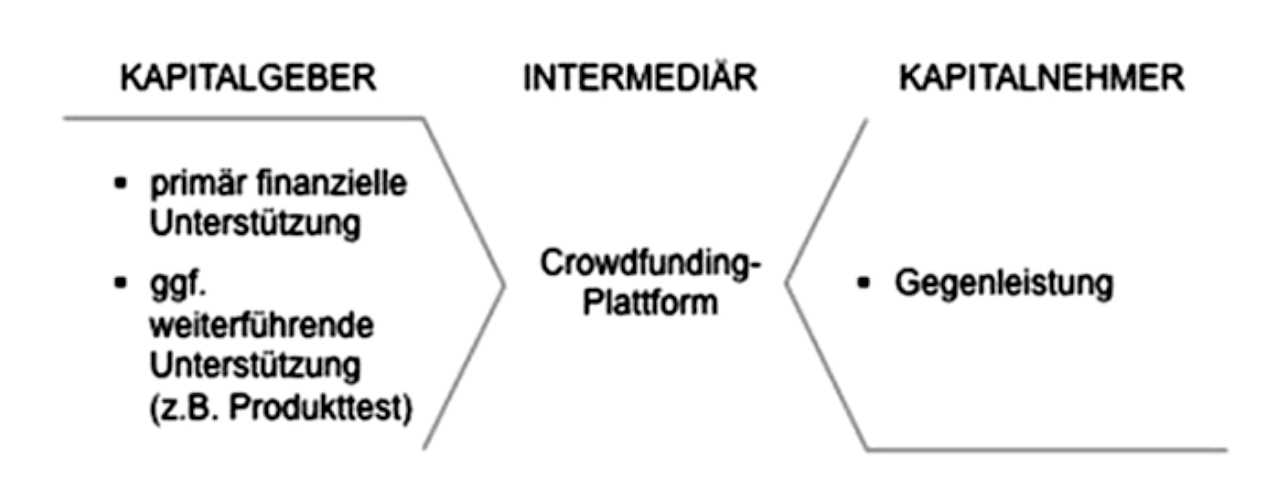
\includegraphics[width=\textwidth]{images/crowdfunding_akteure}
	\caption{Akteure des Crowdfunding-Prozesses. (Quelle: \citeauthor{Guenther2019} \citeyear{Guenther2019})}
	\label{fig:crowdfunding_actors}
\end{figure} 

Der Intermediär bietet für Kapitalnehmer und -geber eine Plattform, auf der mittels eines standardisierten Verfahrens eine Durchführung von Finanztransaktionen gewährleistet wird und ein Informationsaustausch zwischen beiden Parteien hergestellt werden kann \cites[7\psq]{Guenther2019}{moritz2015}.

\subsubsection*{Kapitelnehmer}
Kapitalnehmer, welche im vorliegenden Kontext auch als Projektinitiatoren bezeichnet werden \cite[11]{Gierczak2016}, sind sowohl Einzelpersonen als auch Unternehmen in der Früh- und Spätphase der Geschäftstätigkeit \cites{Gierczak2016}{Schwienbacher2010}[8]{Guenther2019}. Die wichtigste Anforderung aufseiten der Kapitalnehmer ist die überzeugende Darstellung des zu finanzierenden Vorhabens \cites{Guenther2019}{bouncken}. 
\subsubsection*{Intermediär (Plattform)}
Der Intermediär wird als Vermittler des Finanzierungsprozesses angesehen. Dieser stellt dabei standardisierte Prozesse zur Durchführung der Crowdfunding-Kampagnen bereit \cite[9]{Guenther2019}. Die erfolgreiche Kommunikation zwischen Kapitalgeber und -nehmer ist dabei wichtig, um eine Crowdfunding-Kampagne durchzuführen. Seitens der Intermediäre werden diesbezüglich unterschiedliche Transaktionsmechanismen angeboten \cite[9]{Guenther2019}:

\begin{itemize}
	\item ''All-or-Nothing''\newline
	Im Mittelpunkt der meisten Crowdfunding-Plattformen steht das All-or-Nothing Prinzip \cite{cumming_leboeuf_schwienbacher_2014}. Nach diesem Prinzip erhalten Projektinitiatoren den gesammelten Betrag nur dann ausbezahlt, wenn sie ihr vordefiniertes Finanzierungsziel erreichen. Dies beruht auf der Annahme, dass Geldgeber nur dann in der Lage sind ihr Projekt zu verwirklichen und die versprochenen Erträge zu erzielen, wenn sie über die dafür erforderlichen Ressourcen verfügen \cite{Gerber2011Crowdfunding}.
	\item ''Keep-What-You-Get''\newline
	Ein weiterer Transaktionsmechanismus ist das Keep-What-You-Get Prinzip, bei dem die Projektinitiatoren jede gesammelte Summe erhalten \cite{Gerber2011Crowdfunding}.  Dieses Finanzierungsprinzip wird insbesondere bei gemeinnützigen Projekten oder bei Projekten angewandt, die Crowdfunding als untergeordnete Finanzierungsquelle nutzen \cite[42\psqq]{Gebert2013}.
\end{itemize}

\subsubsection*{Kapitalgeber (Crowd)}
Kapitalgeber sind die Geldgeber auf den Crowdfunding-Plattformen. Entscheidet sich ein Kapitalgeber für die Unterstützung eines Projekts, kann er über den Intermediär eine Zahlung mittels eines Zahlungsdienstleisters tätigen. Bei solchen Transaktionen bleiben die Kapitalgeber und ihre finanziellen Beiträge zueinander anonym \cite[10]{Guenther2019}.

\subsection{Ausgestaltungsarten des Crowdfunding}
In den letzten Jahren sind eine Vielzahl verschiedenster Crowdfunding Finanzierungsmethoden aus dem Boden emporgewachsen. \citeauthor{Guenther2019} bezeichnet die folgenden Modelle als die vier Grundformen des Crowdfundings, wobei sich die finanziellen Modelle im Kern in Fremd- und Eigenkapitalfinanzierungen unterscheiden lassen.
\subsubsection*{Fremdkapitalbasiertes (lending-based) Crowdfunding}
Unter dem fremdkapitalbasierten Crowdfunding bzw. Crowdlending wird im deutschen Rechtskreis ein auf Darlehen aufbauendes Finanzierungsmodell verstanden \cite[11]{Guenther2019}. Dabei wird, beim Erreichen des Finanzierungsziels, ein Kreditvertrag zwischen Kreditnehmer und Kreditgebern abgeschlossen. Eine generelle Abbildung des Ablaufs ist in Anhang \ref{sec:A} zu finden.
\subsubsection*{Eigenkapitalbasiertes (equity-based) Crowdfunding}
Beim eigenkapitalbasierten Crowdfunding bzw. Crowdinvesting, investiert die Crowd in Form von Eigen- oder Mezzanine\footnote{Mischform zwischen Eigen- und Fremdkapital \cite{Schrecker2012}}-Kapital in den Kapitalnehmer. Im Gegenzug erhält der Investor Anteile, eine Gewinnbeteiligung oder anderweitig variable Vergütungen \cites[13]{Guenther2019}[195\psq]{Looy2015}. Kurz gefasst handelt es sich in diesem Sinne um eine Beteiligungsfinanzierung.
\subsubsection*{Spendenbasiertes (donation-based) Crowdfunding}
Das spendenbasierte Crowdfunding ist eines der nicht-finanziellen Crowdfunding Modelle. Der Investor, welcher für seine Spende keine Gegenleistung erhält, erfüllt infolgedessen lediglich einen ideellen Zweck. Aus rechtlicher Sicht ist dieses Modell als am wenigsten aufwendig anzusehen, da es auf einer Schenkung basiert. \cite[15\psq]{Guenther2019}
\subsubsection*{Belohnungsbasiertes (reward-based) Crowdfunding}
Eines der ältesten und einfachsten Wege in Crowdfunding-Projekte zu investieren, ist das belohnungsbasierte Crowdfunding, bei welchem der Investor eine vordefinierte Belohnung für sein Investment erhält. Diese Belohnungen sind meist im Umfang eines T-Shirts oder einer ähnlichen Anerkennung. % WTF Grammatik??
 Bei diesem Modell liegt der Schwerpunkt nicht auf dem Erwirtschaften von Gewinnen durch Investments, vielmehr ist die Erfüllung eines guten Zweckes als Beweggrund anzusehen \cites[196]{Looy2015}{Guenther2019}.

\section{Internal Crowdfunding}\label{sec:internal_crowdfunding}
Die Idee des internen Crowdfunding kam auf, als Jurgen Appelo\footnote{Europas beliebtester Autor für Führungspersönlichkeiten (vgl. Inc.com \cites{leadership_experts}{leadership_speakers})} ein großes Entwicklungsteam leitete und versuchte, einen Innovationsausschuss zu schaffen, der die besten Ideen filtern konnte, um neue Projekte voranzubringen. Dieser Ausschuss wurde jedoch von den Ideen überwältigt und konnte nur einige wenige auswählen. Die Mitarbeiter waren entmutigt, als sie das Gefühl hatten, dass ihre Ideen für die Zukunft des Unternehmens ignoriert wurden. Um die Signifikanz der Thematik zu verdeutlichen, wird Appelos Aussage zum internen Crowdfunding genannt:

\begin{quote}
	% https://management30.com/practice/internal-crowdfunding/
	% Einleitung zur Quote herleiten
	% Darauf aufbauen .. 
	\glqq The job of management is not to select the best ideas; it is to create a great system that allows for the best ideas to emerge \cite{appelo2014medium}.\grqq{}
\end{quote}

Internes Crowdfunding ist dabei wie eine Börseninnovation, die es den Mitarbeitern erlaubt, auf Ideen zu bieten, die sie für die Besten halten. Jeder Mitarbeiter kann eine Idee einreichen, muss jedoch die Kollegen von dieser überzeugen. Mitarbeiter erhalten innerhalb eines solchen Systems die Möglichkeit, mit ihrer Stimme oder mit Hilfe von virtueller Währung für ein Projekt zu stimmen, um somit dessen Erfolg zu fördern \cite{management3_internal_crowdfunding}. % Vanderkam noch erklären?
\citeauthor{vanderkam2014}\footnote{Autor zahlreicher Zeitmanagement und Produktivitäts Bücher (vgl. fastcompany.com \cite{vanderkam2014})} begründet hierbei, dass man das Beste aus den Angestellten herausholt, wenn man sie wie Unternehmer behandelt. Wird dem Arbeitnehmer die Möglichkeit gewährt, seine Ideen und Innovationen von den eigenen Kollegen unterstützen zu lassen, fördert dies den Umgang und die einhergehende Akzeptanz der Kollegen untereinander. Gleichzeitig wird dem Unternehmen die Möglichkeit geboten, innovativer zu arbeiten \cite{appelo2014medium}.

%% Noch mehr zu internal Crowdfunding...

% \section{Crowdfunding Risiken}




	
	%!TEX root = ../dokumentation.tex

\chapter{Ist- und Soll-Zustand}
Im Folgenden wird der Kontext der Arbeit durch die Darstellung der Ist- und Soll-Zustände erläutert. Vertiefend zum Soll-Zustand wird die Erzeugung eines Ideen-/Anforderungstickets dargestellt. Abschließend wird mit Hilfe der Anforderungsanalyse ein Soll-Zustand aufgestellt.

\section{Ist-Zustand}
Die Erhebung des Ist-Zustandes erfolgt in Zusammenarbeit mit den Mitgliedern des gegenwärtigen Entscheidungsgremiums. Da der Entscheidungsprozess Abweichungen zwischen den Abteilungen Produktentwicklung sowie Plattformentwicklung aufzeigt, werden diese im Folgenden von einander unterschieden. Zunächst wird die Erstellung eines Tickets im generellen Sinn erläutert.

\subsection*{Generelles Erzeugen eines Ideen-/Anforderungstickets}
Jede Idee bzw. Anforderung, sei sie aus Kunden- oder Mitarbeitersicht, wird auf die gleiche Weise erzeugt. Hierfür wird im camos.SalesCenter\footnote{Plattform zum Anlegen von Tickets} ein neues Ticket erstellt. Diesem wird der Typ \emph{Idee}\footnote{Nicht vorhandenes Feature, welches als nicht kritisch für weitere Arbeit angesehen wird} oder \emph{Anforderung}\footnote{Nicht vorhandenes Feature, jedoch elementar für weitere Arbeit} zugewiesen, um sie im späteren Prozess von einander unterscheiden zu können. Darüber hinaus benötigt jedes Ticket die Zuweisung in eine Produktkategorie. Diese Produktkategorie weist das Ticket dem zugehörigen Entscheidungsgremium zu, welches sich mit der Umsetzung auseinandersetzt. Diesem Ticket können Beitrage hinzugefügt werden, um die Idee bzw. Anforderung zu beschreiben. Mittels der Schaltfläche \emph{Priorität} kann bei Bedarf die Dringlichkeit des Tickets beeinflusst werden. Wird das Ticket von einem Mitarbeiter erstellt und behandelt ein vertrauliches Thema, kann über die Schaltfläche \emph{Sichtbarkeit} das Einsehen von externen Benutzern unterbunden werden. Eine Übersicht der Benutzeroberfläche wird in Abbildung \ref{fig:ticket} dargestellt.

\begin{figure}
	\centering
	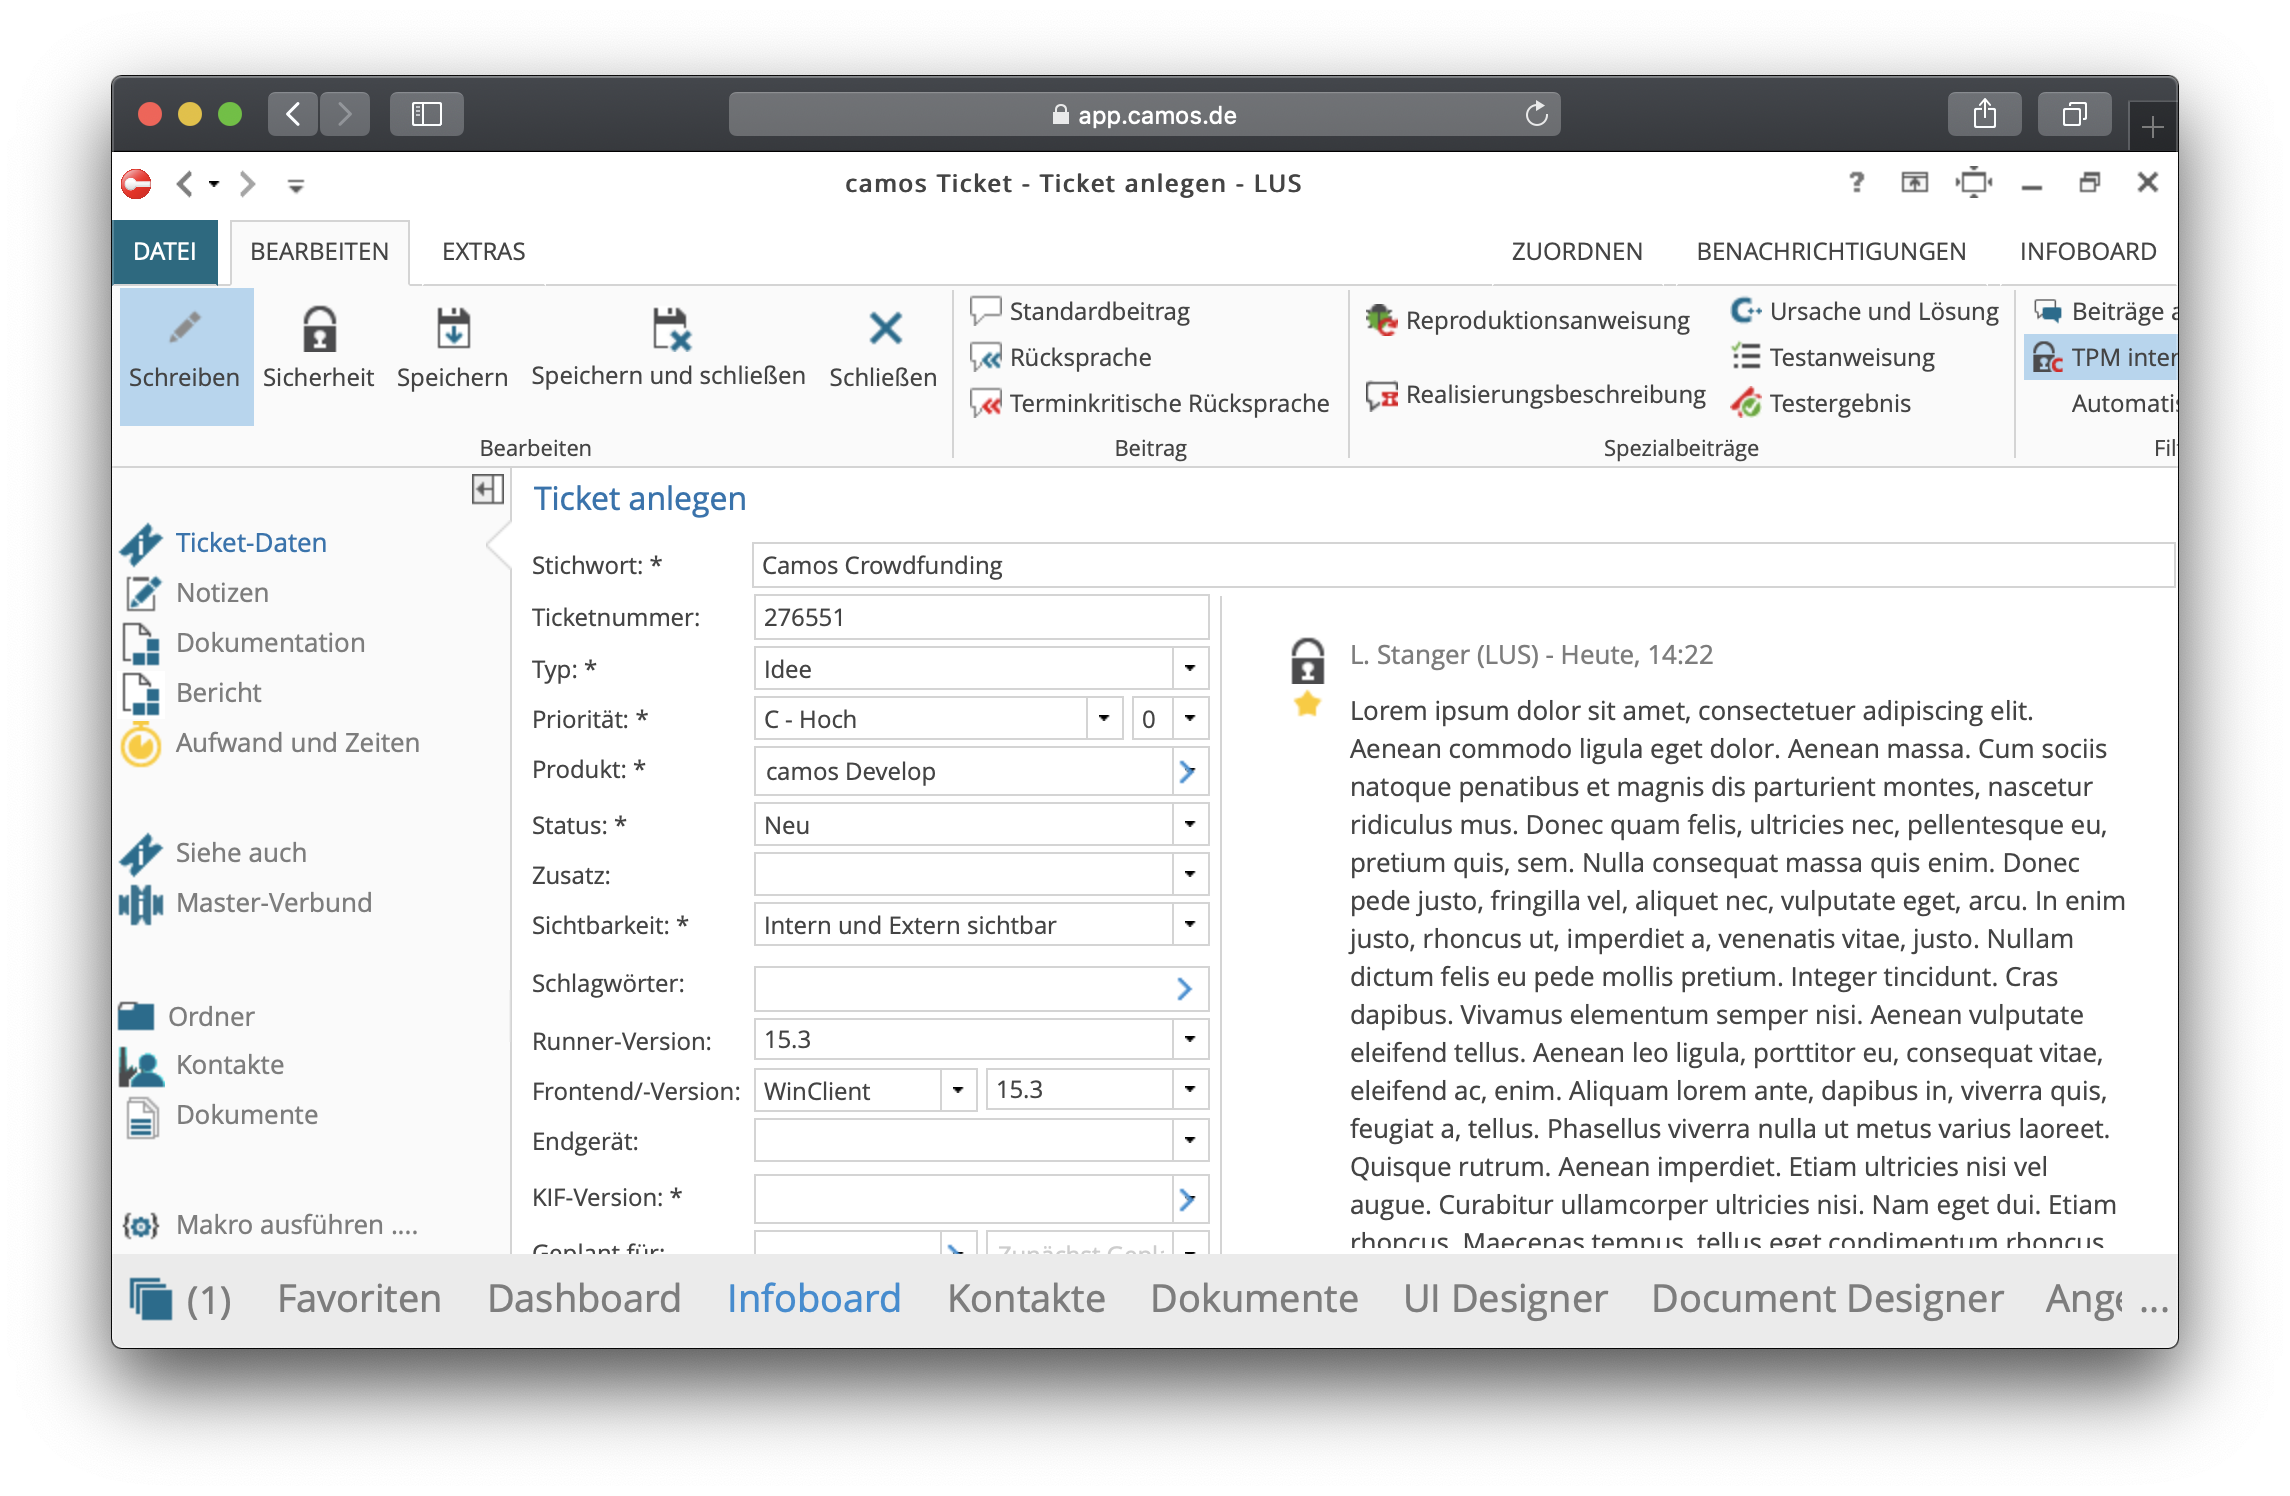
\includegraphics[width=\textwidth]{images/Ticket_erstellen}
	\label{fig:ticket}
	\caption{Benutzeroberfläche zum Erstellen eines Tickets}
\end{figure}

\subsection*{Produktentwicklung Ist-Zustand}
Der Ist-Zustand der Produktentwicklung wurde im Dialog mit einem Mitglied des zugehörigen Entscheidungsgremiums eruiert. Das Gremium bildet sich aus der \ac{GL}, einem \ac{PO} sowie einem erfahrenen Fachexperten und trifft strategische Entscheidungen, wie das Produkt künftig weiterentwickelt wird. Die sich im Ideen-Backlog befindenden Tickets können gleichermaßen von Mitarbeitern sowie Kunden erstellt werden. Der Schlüssel zur Ideen- und Innovationsfindung liegt dabei in der Kommunikation der Dev-Teams, welche ihre täglich gewonnenen Eindrücke aus internen sowie Kunden Projekten in den Prozess einfließen lassen. Als ein weiteres wesentliches Entscheidungskriterium wird die Passgenauigkeit der vorgeschlagenen Idee in die bestehende Strategie gewertet. Die auflaufenden Tickets werden im monatlich abgehaltenen \ac{CPQ}-Gremium diskutiert, bewertet und anschließend in eine Release-Version eingeplant. Sollte es zu einer einstimmigen Ablehnung kommen, wird der Ticketstatus auf abgelehnt gesetzt.

\subsection*{Plattformentwicklung Ist-Zustand}
Im spezifischen wurde der Ist-Zustand in der Plattformentwicklung mit einem Mitglied des dortigen Entscheidungsgremiums erhoben. Im Dialog wurden die Tickets auf die der Plattformentwicklung zugehörigen Produkte beschränkt. Die Abgrenzung wurde hierbei auf die folgenden Produkte vorgenommen:

\begin{itemize}
	\item Laufzeitumgebung camos.Runner
	\item Frontendumgebung camos.WinClient und camos.HTML5Client
	\item Entwicklungsumgebung camos.Develop
	\item Develop-Module camos.LoadBalancer und camos.Scheduler
\end{itemize}

An der Entscheidungsfindung ist, wie zuvor in der Produktentwicklung, ein Gremium beteiligt. Dieses setzt sich aus dem \ac{GL} der Entwicklungsabteilung und den jeweiligen Hauptverantwortlichen der Frontend-, Interpreter- und Plattform-Entwicklung zusammen. Im Rahmen dieses Gremiums werden anhand spezifischer Entscheidungskriterien Tickets aus dem bestehenden Backlog analysiert. Diese Entscheidungskriterien beinhalten einerseits den Fokus auf Großkundenprojekte, andernseits wird versucht, Ideen und Innovationen zur Unterstützung und Weiterentwicklung eines vierteljährlich anstehenden Minor Releases zu erkennen. Tickets, die es nicht in ein kommendes Release geschafft haben, werden stets anhand bestehender Kriterien neu bewertet.

%%Die Umfrage baut sich aus 16 voneinander unabhängigen Fragen auf.
\section{Soll-Zustand}
Für die Aufstellung eines Soll-Zustandes wurde eine firmeninterne Umfrage zum Thema \glqq Möglichkeit und Akzeptanz einer internen Crowdfunding Plattform bei camos\grqq{} durchgeführt. Die daraus erhobenen Erkenntnisse fließen direkt in den Soll-Zustand ein.

\subsection{Aufbau der Umfrage}\label{sec:AufbauUmfrage}
Als Umfragetool wurde sich für die von Google LLC entworfene Lösung Google Forms entschieden. Ausschlaggebend für die Verwendung war die kostenlose Nutzung des Tools sowie die leichte Bedienbarkeit mit weitreichenden Gestaltungsmöglichkeiten der einzelnen Fragen. Die Umfrage setzt sich aus 16 Fragen zusammen, welche initial die bereits vorhandene Kenntnis bezüglich der Themengebiete Crowdfunding und internem Crowdfunding aufnimmt. Weitergehend wird die Akzeptanz und Verwendung des gegenwärtigen Ideen- und Innovationsprozesses examiniert. Dem Umfrageteilnehmer wird im Anschluss die Möglichkeit geboten, Bedenken sowie eigene Interessen im Zusammenhang mit einer internen Crowdfunding Plattform zu nennen. Zuletzt werden Themengebiete erhoben, die mithilfe dieser Plattform behandelt werden sollen. Ziel der Umfrage ist es, die Meinung aller Mitarbeiter, unabhängig ihrer Position zu erfassen und daraus ein auf die Anforderungen angepasstes Konzept zu schaffen. Die Umfrage wird allen beschäftigten Mitarbeitern für einen Monat zur Verfügung gestellt.

%TODO: Umfrage als PDF einfügen.

\subsection{Auswertung der Umfrage}\label{sec:Umfrageauswertung}

Von den befragten 120 Mitarbeitern haben 75 Mitarbeiter an der Umfrage teilgenommen. Um ähnliche Antworten gruppieren zu können, wurde zunächst die Abteilung mit der derzeit ausgeübten Position abgefragt. Als erste themenrelevante Frage wurde der Kenntnisstand des gegenwärtigen Ideen-Einreichungsprozesses abgefragt. Darunter hat sich eine Gruppe von 29 Mitarbeitern (38,7\%) ergeben, die den gegenwärtigen Prozess nicht kennt, wohingegen 46 Mitarbeiter (61,3\%) die Kenntnis am Prozess bejahen. Diese Kennzahl zeigt schon zu Beginn der Umfrage dringenden Handlungsbedarf bezüglich des Ideen- und Innovationsprozess auf. Daraus lässt sich die \ac{NFA}-1 ableiten - \emph{Klare Definition des Ideen- und Innovationsprozesses}. Weitergehend wurde der Kenntnisstand des Auswahlprozesses für neue Ideen abgefragt, welchen 60 Mitarbeiter (80\%) als nicht geläufig bezeichnet haben. Dies bringt \ac{NFA}-2 hervor - \emph{Transparenz des Prozesses zur Entscheidung neuer Ideen und Innovationen}. Da keine Kennzahl zur gegenwärtigen Verwendung des Prozesses vorliegt, wurde diese, unter Verwendung der in Abbildung \ref{fig:frage4} aufgeführten Frage, erhoben. Daraus ist abzuleiten, dass 32 Mitarbeiter (42,7\%) noch nie die Möglichkeit ergriffen haben, eine Idee im Ticketsystem einzustellen. 
\begin{figure}[]
	\centering
	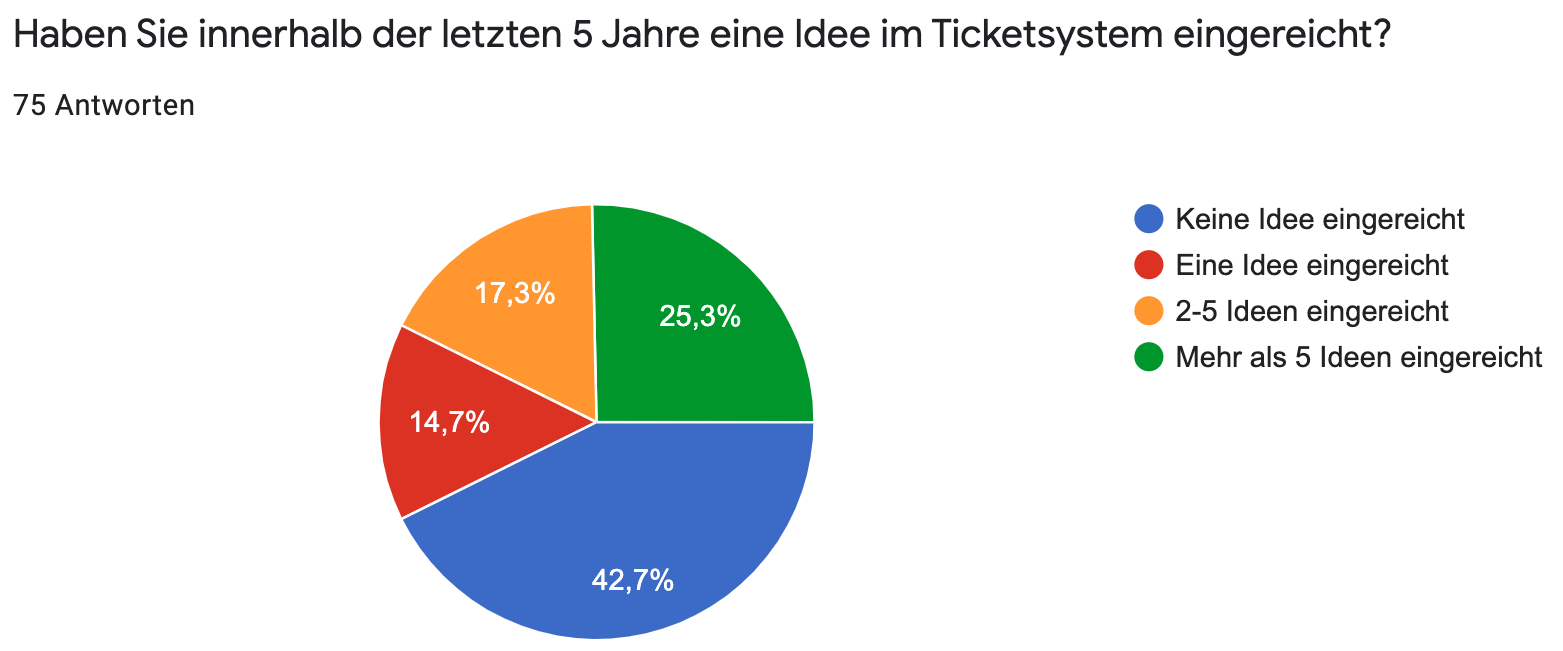
\includegraphics[width=\textwidth]{images/Frage4}
	\caption{Erhebung einer Verwendungskennziffer des gegenwärtigen Prozesses}
	\label{fig:frage4}
\end{figure} 
Durch Auswertung der zuvor angegebenen Abteilung ist zu erkennen, dass die Antwortmöglichkeit \emph{Mehr als 5 Ideen eingereicht} vornehmlich von Mitarbeitern der Beratungs- und Entwicklungsabteilung getroffen wurde. Ein eindeutiger Trend bei der Antwortmöglichkeit \emph{Keine Idee eingereicht} ist in der Abteilungsgruppierung HR/Vertrieb/Verwaltung zu erkennen, was einerseits mit der Fremdheit der Produktpalette zu erklären ist, andererseits hat, wie in Kapitel \ref{sec:internal_crowdfunding} erwähnt, jeder Mitarbeiter ein Potential an Ideen und Innovationen. Da dieses Potential mutmaßlich verloren geht, soll mit Hilfe von \ac{NFA}-3 - \emph{Keine Beschränkung der Ideen und Innovationen auf Produkte} - produktfremden Mitarbeitern eine Möglichkeit der Ideen- und Innovationspublikation geschaffen werden. Von den 43 Mitarbeitern, die innerhalb der letzten fünf Jahre \emph{mindestens} eine Idee eingereicht haben, gaben elf an, dass sie nicht wissen, was mit ihren Ideen passiert. Um dies in einem verbesserten Prozess zu verhindern, soll durch die \ac{FA}-1a - \emph{Benachrichtigung bei Akzeptanz einer Idee} bzw. \ac{FA}-1b - \emph{Benachrichtigung bei Verwerfung einer Idee} mehr Transparenz in den Entscheidungsverlauf gebracht werden. Damit neben dem gegenwärtig verwendeten Prozess die Geläufigkeit des Themas Crowdfunding eingeschätzt werden kann, wurde unter Verwendung einer linearen Skala von 1 - \emph{Ja, ich weiß was der Begriff bedeutet} bis 5 - \emph{Nein, ich weiß nicht was der Begriff bedeutet} eine Kennzahl diesbezüglich eingeholt. Eine kumulierte Anzahl von 11 Mitarbeitern (14,7\%) haben hierbei eine \glqq{}3\grqq{} oder schlechter vergeben. Folglich sollte eine Erläuterung des Begriffs \emph{Crowdfunding} stattfinden, um die Zahl der Mitarbeiter zu minimieren. Zusätzlich zu dieser Erläuterung sollte der Unterschied zwischen Crowdfunding und internem Crowdfunding geklärt werden, da die überwiegende Mehrheit (76\%) angegeben hat, keine Kenntnisse bezüglich des internen Crowdfundings zu besitzen. Dessen ungeachtet ist die Akzeptanz an eine interne Crowdfunding Plattform und die damit einhergehende Modifikation des gegenwärtigen Prozesses mit 62 Ja-Stimmen (82,7\%) deutlich vorhanden. 
\begin{figure}[t]
	\centering
	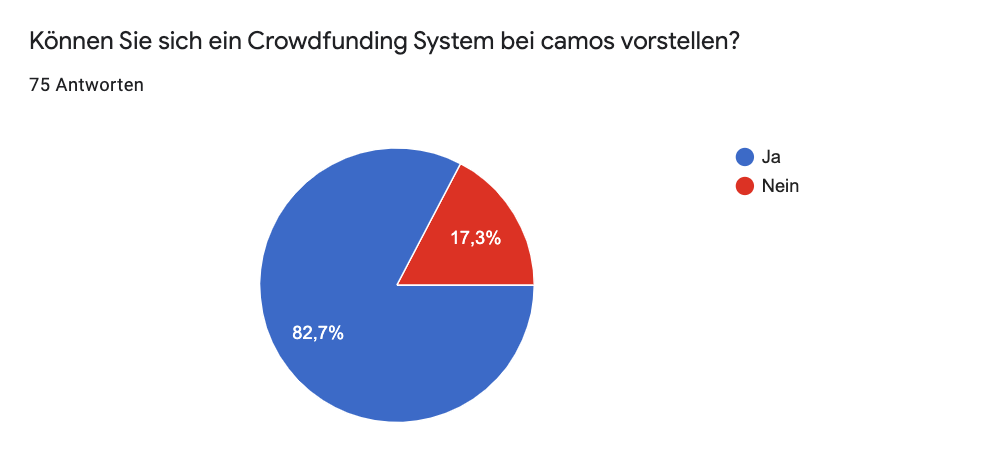
\includegraphics[width=\textwidth]{images/Frage9}
	\caption{Validierung der Akzeptanz einer Prozessänderung}
	\label{fig:frage9}
\end{figure} 
Mit ein Grund hierfür ist das Resultat der in Abbildung \ref{fig:frage7} aufgeführten Frage. Hieraus lässt sich erkennen, dass lediglich 10 Mitarbeiter (13,3\%) der Ansicht sind, dass die besten Ideen den Weg in das Produkt finden. Auf der anderen Seite jedoch, wurde von 26 Mitarbeitern (34,7\%) die Ansicht geäußert, dass gute Ideen teilweise nicht wahrgenommen werden. Die von über einem Drittel der Umfrageteilnehmer getroffene Aussage, dass der gegenwärtige Prozess gute Ideen teilweise nicht wahrnimmt, unterschreibt erneut die Dringlichkeit einer Prozessüberarbeitung. Auf die Frage, ob bereits eine Ticketidee des Umfrageteilnehmers für ein internes Crowdfunding System vorhanden ist, hatten nur 19 Mitarbeiter (25,3\%) mit \glqq{}Ja\grqq{} abgestimmt. 
\begin{figure}[b]
	\centering
	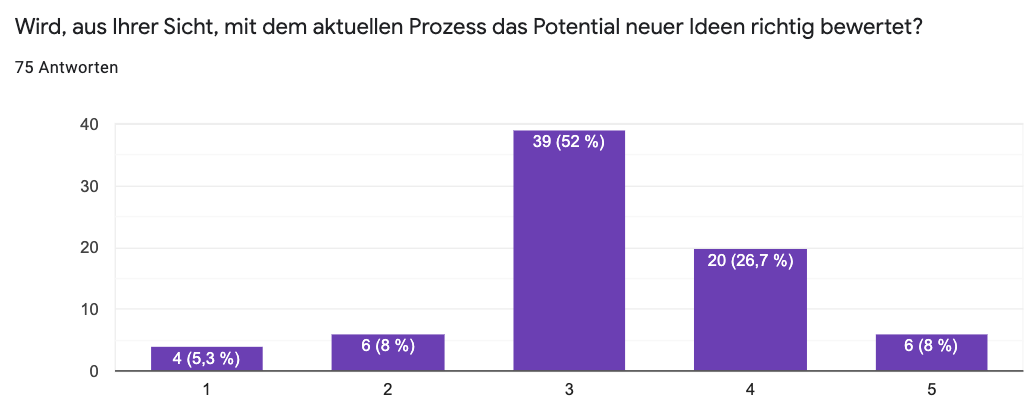
\includegraphics[width=\textwidth]{images/Frage7}
	\caption{Gegenwärtige Ansicht bezüglich des Entscheidungsprozesses}
	\label{fig:frage7}
\end{figure} 
In Kombination mit der Frage, ob ein Belohnungssystem für erfolgreich umgesetzte Ideen eingeführt werden sollte, welche die Mehrzahl der Mitarbeiter (60\%) bejaht haben, lässt sich durch \ac{FA}-2 - \emph{Belohnungssystem} ein Stimulus bezüglich der zukünftigen Teilnahmequote setzen. Um darüber hinaus funktionale sowie nicht-funktionale Aspekte der zukünftigen Lösung erheben zu können, wurden mithilfe einer Multiple-Choice Umfrage zunächst vorgegebene Aspekte der Bewertung unterzogen. Dabei wurden die vorgegebenen Aspekte grundlegend als Positiv bewertet. Aufgrund der positiven Resonanz resultieren \ac{FA}-3 - \emph{Mobile Erreichbarkeit der Plattform} sowie \ac{FA}-4 - \emph{Keine quantitative Begrenzung der Ideenerstellung}. Weitergehend wird die Zusammenführung von Ideentickets, welche den gleichen Inhalt beschreiben, gefordert. Dies soll durch \ac{FA}-5 - \emph{Zusammenführung von Tickets} gewährleistet werden. Als ein weiterer maßgeblicher Aspekt wurde die Filtermöglichkeit von Ideentickets bewertet, um interessante Tickets für den Anwender einfacher auffindbar zu machen. Um die Umsetzung dieses Aspekts sicherzustellen, wird \ac{FA}-6 - \emph{Filtermöglichkeit von Ideentickets} aufgestellt. Als wichtigster Aspekt wurde, seitens der Umfrageteilnehmer, die gleichwertige Gewichtung von Stimmabgaben, unabhängig der Position des Mitarbeiters, gewählt. Dies soll mithilfe von \ac{NFA}-4 - \emph{Gleichwertige Gewichtung der Stimmen} sichergestellt werden. Über die Bewertung der vorgegebenen Aspekte hinaus, haben sich weitere Faktoren ergeben, die den Umfrageteilnehmern wichtig sind. Diese wurden durch die Möglichkeit einer Freitext Eingabe erhoben, woraus sich \ac{FA}-7 - \emph{Feedback über Status einer Idee}, \ac{FA}-8 - \emph{Möglichkeit der Kommentierung einer Idee}, \ac{FA}-9 - \emph{Sichtbarkeit der Stimmen} - sowie \ac{FA}-10 - \emph{Anonyme Abstimmungsmöglichkeit} ergeben. Abschließend wurde der Umgang mit älteren und noch nicht realisierten Ideentickets erfasst, welcher von 44 Mitarbeitern (62,9\%) mit \emph{Das Ziel wurde nicht erreicht. Für eine zweite Chance muss die Idee reaktiviert werden} - abgestimmt wurde. Daraus entsteht \ac{NFA}-5 - \emph{Abgelaufene Ideentickets müssen reaktiviert werden}.
\begin{figure}[hb]
	\centering
	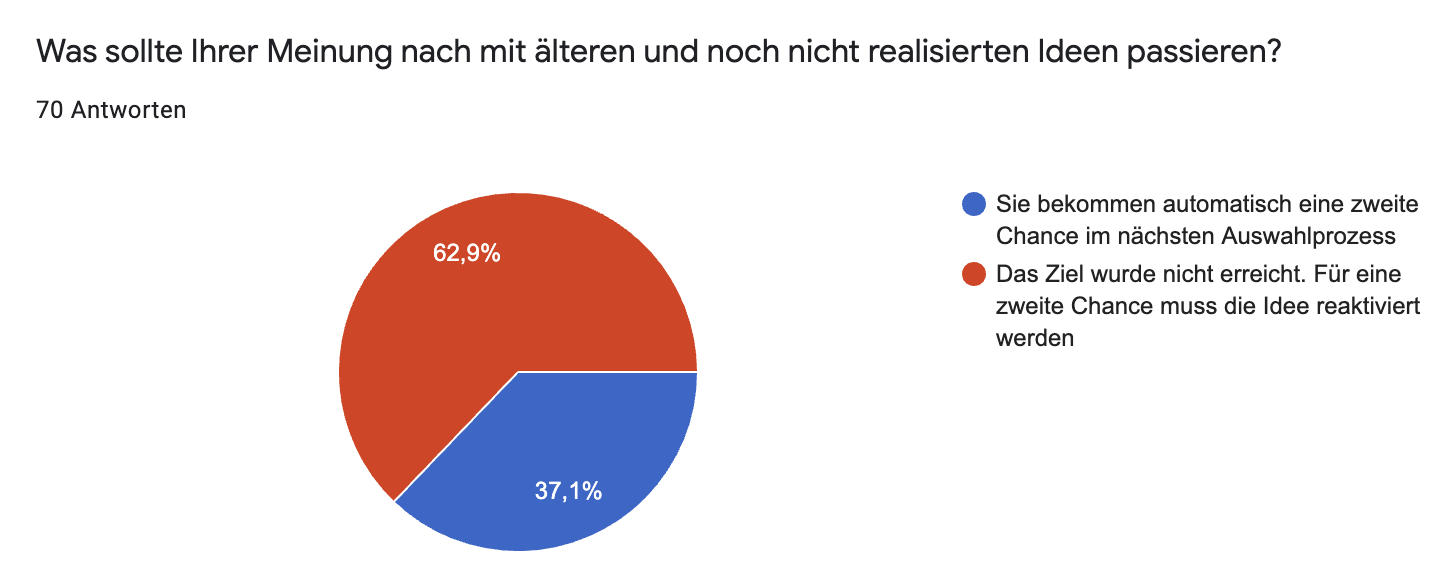
\includegraphics[width=\textwidth]{images/Frage16}
	\caption{Umfrageergebnis der Handhabung abgelaufener Ideentickets}
	\label{fig:frage16}
\end{figure} 
\newpage
\subsection{Tabellarische Aufstellung der erhobenen Anforderungen}\label{sec:anforderungen_tabellarisch}

\begin{longtable}[h]{|l|p{10cm}|}
\hline
Anforderungskennzeichen & Anforderungskurzbeschreibung \\
\hline
FA-1\label{itm:FA-1} & Als Anwender möchte ich bei Akzeptanz einer Idee informiert werden.\\
\hline
FA-2 & Als Anwender möchte ich für konstruktive Ideen belohnt werden.\\
\hline
FA-3 & Als Anwender möchte ich die Crowdfunding Plattform mobil erreichen können.\\
\hline
FA-4 & Als Anwender möchte ich nicht durch eine quantitative Einschränkung der Ideen begrenzt werden.\\
\hline
FA-5 & Als Anwender möchte ich Ideentickets mit ähnlichem Inhalt zusammenführen können.\\
\hline
FA-6 & Als Anwender möchte ich ausgiebige Filtermöglichkeiten erhalten, um Tickets meines Interessengebiets leichter ausfindig zu machen.\\
\hline
FA-7 & Als Anwender möchte ich Feedback über den Status einer Idee erhalten.\\
\hline
FA-8 & Als Anwender möchte ich für mich relevante Ideen kommentieren können.\\
\hline
FA-9 & Als Anwender möchte ich stets die Anzahl der Stimmen einsehen können, die eine Idee unterstützen.\\
\hline
FA-10 & Als Anwender möchte ich die Möglichkeit haben, Ideen anonym unterstützen zu können.\\
\hline
NFA-1 & Der Ideen- und Innovationsprozess muss klar definiert sein.\\
\hline
NFA-2 & Der Entscheidungsprozess von Ideen und Innovationen muss transparent einsehbar sein.\\
\hline
NFA-3 & Ideen und Innovationen dürfen nicht auf Produktebene beschränkt werden.\\
\hline
NFA-4 & Stimmabgaben müssen zu jeder Zeit, unabhängig der Position des Mitarbeiters, gleich gewichtet werden. \\
\hline
NFA-5 & Wird ein Ticket in einer vorbestimmten Zeit nicht umgesetzt muss es vom Ersteller reaktiviert werden. \\
\hline
\caption{Tabellarische Auflistung funktionaler und nicht funktionaler Anforderungen}\label{tab:Anforderungsanalyse}
\end{longtable}












	
	%!TEX root = ../dokumentation.tex
%%%%%%%%%%%%%%%%%%%%%%%%%%%%%%%%%%%%%%%%%%%%%%%%%%%%%%%%%%%%%%%%%%%%%%%%%%%%%%%%%%%%%%%%%%%%%%%%%%%%%%
%% Tabledefinition
\newcommand{\mc}[2]{\multicolumn{#1}{c}{#2}}
\definecolor{Gray}{gray}{0.85}
\definecolor{CamosRed}{rgb}{0.76, 0.08, 0.067}

\newcolumntype{a}{>{\columncolor{Gray}}c}
\newcolumntype{b}{>{\columncolor{white}}c}
%% End Tabledefinition
%%%%%%%%%%%%%%%%%%%%%%%%%%%%%%%%%%%%%%%%%%%%%%%%%%%%%%%%%%%%%%%%%%%%%%%%%%%%%%%%%%%%%%%%%%%%%%%%%%%%%%
\chapter{Konzeption}\label{sec:concept}
Im Folgenden wird die Konzeption der camos Crowdfunding Lösung behandelt. Hierbei wird eine Veranschaulichung des Konzepts beabsichtigt. Darüber hinaus wird die Möglichkeit einer Umsetzung mittels einer bereits etablierten Softwarelösung analysiert.

\section{Inhalte des Konzeptes}
Um eine einheitliche Definition für das Konzept zu schaffen, werden initial die einzelnen Bestandteile definiert. Grundlegend muss das Konzept alle zuvor in Kapitel \ref{sec:anforderungen_tabellarisch} aufgeführten Anforderungen erfüllen. Um den Funktionsumfang der Crowdfunding Lösung definieren zu können, wird der Prozess anhand bestehender Kriterien abgegrenzt. Durch diese Abgrenzung wird vermieden, dass das eigentliche Ziel der Lösung verfehlt wird.

\section{Abgrenzung camos Crowdfunding}
%TODO: Abgrenzung?!
Das Überarbeiten eines bestehenden Prozesses kann schnell über das Ziel hinausschießen oder es gänzlich verfehlen. Um dies zu vermeiden wird im Folgenden eine Abgrenzung der Prozessmodifikation vorgenommen.

Die camos Crowdfunding Lösung soll ein nicht-autarkes System zur Verbesserung des Ideen- und Innovationsprozesses darstellen. Das eingeführte System muss, neben den Ideen und Innovationen der eigenen Mitarbeiter, die Interessen und Belangen der Kunden berücksichtigen und somit ein Geflecht aus internem Crowdfunding und Open Innovation bilden. Ein direkter Zugang des Kunden zum System ist nicht gewünscht, weshalb eine Integration in das bestehende System notwendig ist. Unterstützend zum gegenwärtigen Prozess, sollen Ideen und Innovationen durch die Plattform anonym \emph{sichtbar} gemacht werden und den Entscheidungsgremien der Produkt- und Plattformentwicklung bereitgestellt werden.

Durch die Einführung der Crowdfunding Plattform und der einhergehenden Öffnung des Innovationsprozesses wird eine Modifikation des belohnungsbasierten Crowdfundings beabsichtigt. Die Mitarbeiter sollen durch die Bereitstellung einer virtuellen Währung eigene Ideen publizieren und gleichzeitig ihre Interessen unterstützen können. Als Stimulus soll eine zu definierende Belohnung für konstruktive Ideen eingeführt werden.

\section{Umsetzung mit Cultivate Labs Ignite}\label{sec:ignite}
Da auf dem Markt für Internes Crowdfunding bereits eine etablierte Lösung existiert, wird zunächst die Umsetzbarkeit mittels dieser analysiert. Die Software Ignite von Cultivate Labs ist eine speziell für das interne Crowdfunding entwickelte Plattform, die sich auf dem internationalen Markt bei einer Vielzahl von Kunden bewährt hat. Um die Umsetzbarkeit zu bewerten, werden die zuvor definierten Anforderungen mit dem Ignite Portfolio abgeglichen. Nach näherer Recherche hat sich herausgestellt, dass die Ignite Plattform viele Funktionen besitzt, jedoch die aus der Umfrage erhobenen Anforderungen nicht gänzlich erfüllt. Die mobile Erreichbarkeit der Plattform konnte über das Portfolio nicht gewährt werden, woraufhin eine Anfrage bei Cultivate Labs eingegangen ist, um diese Frage zu beantworten. Nach Rückantwort wurde bestätigt, dass die Mobile Erreichbarkeit derzeit nicht möglich ist und auch nicht in naher Zukunft geplant sei. Darüber hinaus sei das Zusammenfügen von Ideentickets, wie es in \ac{FA}-5 gefordert wird, nicht umsetzbar. Weitergehend ist die Auswahl von Währungen auf die Selektion von Geld begrenzt. Neutrale Währungen wie Stimmen werden nicht angeboten, was schlussendlich zum Ausschluss der Software führt. Trotz der Möglichkeit, die nicht genannten Anforderungen umzusetzen, bilden die zuvor genannten Kriterien gemeinsam einen ausschlaggebenden Grund, die Software nicht zu verwenden.

\newpage

\section{Konzeption camos Crowdfunding}\label{sec:c_crowd}
Aufgrund der nicht ausreichenden Konfigurationsmöglichkeiten seitens der Software Ignite, muss eine Lösung innerhalb der camos eigenen Programmierumgebung konzipiert werden. Die Verwendung der \ac{DSL} camos.Develop wird hierbei in Betracht gezogen, da das akquirierte Wissen innerhalb des Unternehmens dem einer \ac{GPL} überwiegt. Durch das Entwerfen einer eigenen Software wird darüber hinaus die Möglichkeit geschaffen, sie auf den eigenen Serverlandschaften des Unternehmens zu hosten, sowie jegliche Anforderungen spezifisch umzusetzen. Gleichzeitig ist die Integration in den gegenwärtigen Prozess durch die Verfügbarkeit interner Schnittstellen vereinfacht. 

Zu Beginn muss die Entscheidung für eine Plattform getroffen werden. Hierfür kommt einerseits der camos.WinClient in Frage, welcher die Entwicklung auf Desktop-Geräten unter Verwendung des Betriebssystems Windows ermöglicht. Andererseits kann auf den camos.HTML5Client zurückgegriffen werden, welcher plattformunabhängig in einem unterstützten Webbrowser läuft. Mit Hilfe der camos.Develop IDE lässt sich die Software simultan für beide Plattformen entwickeln. Es sollte hierbei jedoch der Fokus auf den camos.HTML5Client gesetzt werden, da durch \ac{FA}-3 die mobile Erreichbarkeit der Anwendung sichergestellt werden muss. Durch die native Unterstützung von Mobilgeräten im HTML5Client wird die Einhaltung der mobilen Erreichbarkeit gewahrt. Auf Grund der breiten Schnittstellenverfügbarkeit innerhalb der camos eigenen Produktlinie, kann die camos Crowdfunding Lösung direkt in den gegenwärtigen Prozess integriert werden. Hierdurch kann mittels der camos.Ticket Schnittstelle die Crowdfunding Plattform zum Intermediär des Prozesses werden. Dabei wird ermöglicht, Kundenmeinungen in den Prozess einzubinden, ohne ihnen direkten Zugriff auf die Crowdfunding Plattform zu gewähren. Dies wird arrangiert, indem Kundenanforderungen nach wie vor in camos.Ticket aufgenommen, jedoch nach ausreichender Prüfung in das Crowdfunding System übergeben werden können.

In Anbetracht der Tatsache, dass der Ideen- und Innovationsprozess nachgewiesenermaßen durch die Unsicherheit einiger Mitarbeiter beeinflusst wird, sollen Votes anonymisiert werden. Hierdurch soll diesen Mitarbeitern die Chance gegeben werden, nicht für ihre Meinung diskreditiert zu werden. Gleichermaßen geht damit die Erfüllung von \ac{FA}-10 einher. Weitergehend ist unter Beachtung von \ac{FA}-8 die Möglichkeit, Kommentare zu einzelnen Ideen erstellen zu können, einzuführen. Da diese die Meinung des Mitarbeiters vertreten, sollte das Verfassen eines Kommentars nicht anonymisiert werden. Um die Transparenz in Bezug auf den Status einer Idee gewährleisten zu können, soll mit Hilfe eines UI-Elements Plastizität geschaffen werden. Dieses Element soll die zugehörige Zahl der Unterstützer anzeigen. Damit dem Nutzer die Maximierung des Informationsflusses ermöglicht wird, soll unter Berücksichtigung von \ac{FA}-7 die Möglichkeit eingeführt werden, Ideen zu abonnieren, um somit über Änderung bzw. Akzeptanz der jeweiligen Idee informiert zu werden. 

Zur Wahrung der Übersichtlichkeit und um Ideen mit gleicher Absicht gruppieren zu können, soll eine Option zur Zusammenführung von Ideen implementiert werden. Sollte dabei der Fall auftreten, dass beide Ideen bereits Unterstützer haben, wird die Idee mit der Mehrzahl der Stimmen präferiert und im weiterführenden Verlauf als \emph{Master-Idee} gehandhabt. Ein weiterer Aspekt zur Wahrung der Übersichtlichkeit ist eine ausgiebige Filtermöglichkeit. Im Dialog mit den Stakeholdern wurde darauf hingewiesen, dass das \emph{einfache} Finden von Ideen eine große Rolle spielt, da bei einer unübersichtlichen Anzahl von Ideen der Überblick leicht verloren gehen kann. Ist es einer Idee nicht gelungen, in einem bestimmten Zeitraum ausreichend Unterstützer zu sammeln, wird dieser der Status \emph{abgelaufen} zugewiesen. 

\begin{figure}[h]
	\centering
	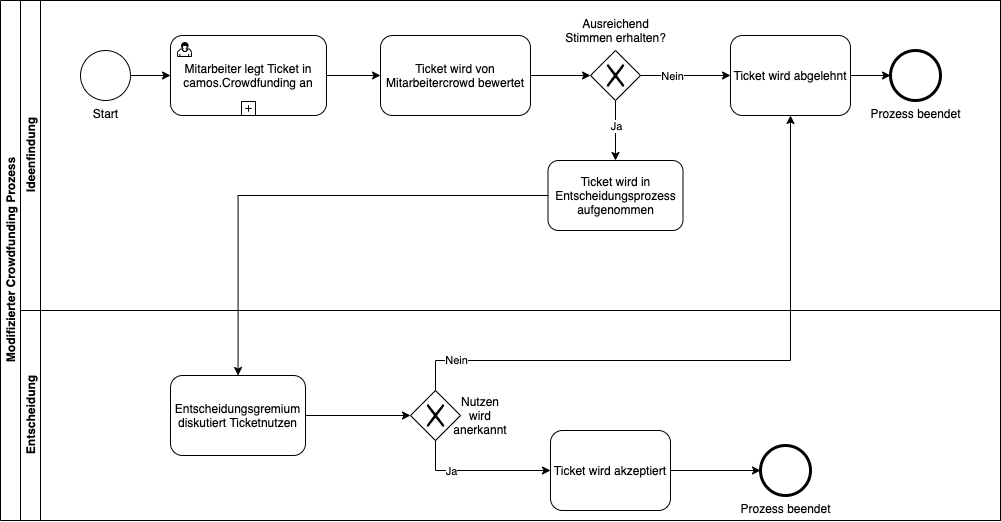
\includegraphics[width=\textwidth]{images/ProcessBPMN}
	\caption{Modifizierter Crowdfundingprozess}
	\label{fig:processbpmn}
\end{figure} 

\newpage
\subsection*{Integration in den gegenwärtigen Prozess}
Um die Plattform in ihrem zuvor beschrieben Umfang in den gegenwärtigen Prozess einbinden zu können, müssen weitergehend die in Tabelle \ref{tab:Anforderungsanalyse} aufgeführten \acs{NFA} berücksichtigt werden. Ausschlaggebend hierfür ist, die in \ac{NFA}-1 erhobene, klare Definition des Ideen- und Innovationsprozesses. Dies ist notwendig, da in Anbetracht der durchgeführten Umfrage eine Vielzahl an Mitarbeitern keine bzw. wenige Berührungspunkte mit einer unternehmensinternen Crowdfunding Lösung hatten. Um daher die Akzeptanz an eine solche Lösung zu steigern, muss die Definition des modifizierten Entscheidungsprozesses kommuniziert werden. Als Kommunikationskanal dienen die \ac{GL} und Entscheidungsgremien. Über die Definition des Prozesses hinaus, wurde von einer Vielzahl an Mitarbeitern Transparenz bezüglich der Entscheidungskriterien gewünscht. Hierbei bedarf es einer spezifischen Definition der Entscheidungskriterien, welche über einen auszuwählenden Kommunikationskanal kontinuierlich an die Mitarbeiter weitergeleitet werden. Um weitergehend Ideen und Innovationen nicht, wie im gegenwärtigen Prozess, auf Produktebene einzuschränken, sollen Mitarbeiter Ideen und Innovationen zu jeglichen Themengebieten aufstellen können. Dies fördert insbesondere passiv den Erfindergeist des einzelnen Mitarbeiters, da ihm unterbewusst die Möglichkeit der Partizipation angeboten wird. Um die Wertschätzung innerhalb des Entscheidungsprozesses nicht zu beeinträchtigen, müssen die Stimmen aller Mitarbeiter, unabhängig ihrer Position grundsätzlich gleich bewertet werden. Die Missachtung dieser Richtlinie würde sich andernfalls in einer Demoralisierung der teilnehmenden Crowd widerspiegeln, da durch ein Ungleichgewicht der Stimmwertung die Exklusivität der individuellen Stimme verloren geht. 







	
	%!TEX root = ../dokumentation.tex
	
	%!TEX root = ../dokumentation.tex
\chapter{Abschluss}
Im Folgenden wird der Abschluss dieser Arbeit dargestellt. Die Vorteile einer eigenständig entworfenen Software gegenüber der marktetablierten Ignite Lösung wurden dargelegt, dabei wurde ein Vorschlag für die konzeptionelle Umsetzung unter Berücksichtigung aller Anforderungen erstellt. Weitergehend wird ein Fazit aus den gewonnenen Erfahrungen bezüglich der Konzeption entnommen.
\section{Fazit}
Aus Kapitel \ref{sec:concept} geht hervor, dass das erarbeitete Konzept technisch möglich und durchführbar ist. Um das Konzept als erfolgreich werten zu können, muss eine weitergehende Evaluierung statt finden, welche die prozessbeteiligten Personen mit einbezieht. Im Rahmen der Konzeption wurde auf die aus der Umfrage erhobenen Bedenken eingegangen. Komplexeren Bedenken wurden Lösungsansätze entgegengebracht, die jedoch dem Zeitpunkt der Implementierung und dessen Stand der Technik angepasst werden müssen. Hierbei ist zu erwähnen, dass die dargestellten Umsetzungsvorschläge lediglich Varianten offenlegen und bei einer evidenten Umsetzung gegebenenfalls modifiziert werden müssen.

Um dem Funktionsumfang von etablierten Crowdfunding Lösungen, wie zum Beispiel Kickstarter und Indiegogo, entsprechen zu können, sind weitere Untersuchungen notwendig. Einerseits muss abgewägt werden, ob bei der Implementierung einer eigenen Crowdfunding Lösung der Aspekt der Kernkompetenzen von camos nicht überschätzt wird und ob somit eine Implementierung überhaupt wirtschaftlich tragbar ist. Der Versuch, eine eigene und unabhängige Crowdfunding Lösung zu bieten, welche Mitarbeiter und Geschäftsleitung gleichermaßen zufriedenstellt, geht mit Schwierigkeiten einher. So müssen auf der einen Seite die gestellten Anforderungen berücksichtigt werden, auf der anderen Seite darf der Standpunkt der gegenwärtigen Entscheidungsgremien nicht gänzlich ignoriert werden. Die Umsetzung dieser Anforderungen bedarf einiger Zeit in der Implementierung und Pflege. In Anbetracht dessen, muss die Frage beantwortet werden, ob eine externe Lösung unter Modifikation des eigenen Prozesses die bessere Lösung wäre. Die Entwicklung dieser externen Crowdfunding Lösungen erfährt meist den vollen Fokus der jeweiligen Anbieter und dementsprechend der Entwicklungskapazitäten. Hieraus resultiert, dass eine Abwägung von Aufwand und Nutzen vorgenommen werden muss. 

\section{Ausblick}

Durch die in dieser Arbeit gestellte Umfrage und des daraus hervorgehenden Konzepts ist die Akzeptanz einer Crowdfunding Lösung analysiert. Es wäre darüber hinaus lohnenswert, das Konzept zu evaluieren. Hierfür kann den Mitgliedern der Entscheidungsgremien, sowie den Geschäftsleitern, ein Evaluierungsbogen zugesandt werden, indem das erhobene Konzept auf seine Vollständigkeit geprüft wird. Die daraus gewonnenen Erfahrungen können, in näherer Zusammenarbeit mit der Geschäftsleitung, in eine überarbeitete Version des Konzepts einfließen. 

Wie schon zuvor in Kapitel \ref{sec:concept} erwähnt, ist es für die erfolgreiche Implementierung einer Crowdfunding Plattform elementar, der Mitarbeitercrowd den Nutzen hinter dieser Plattform darzulegen. Zur Aufklärung kann ein dafür vorgesehenes Dokument angefertigt werden, welches die Modifikation des Prozesses transparent darstellt und für jeden Mitarbeiter zu jeder Zeit verfügbar ist. Über den Umfang dieser Arbeit hinaus wird das Konzept intern weiterentwickelt, um in naher Zukunft einen ersten Prototypen verwenden zu können.


	\clearpage

	% Literaturverzeichnis
	\cleardoublepage
	\printbibliography

	% Glossar
	\printglossary[style=altlist,title=\langglossar]
	
	% sonstiger Anhang
	\clearpage
	\appendix
	% !TeX root = ../dokumentation.tex
\begin{appendix}

\addchap{\langanhang}

{\Large
\begin{enumerate}[label=\Alph*.]
	\item Anhang 1: Funktionsweise Crowdlending
\end{enumerate}
}
\pagebreak
%\includepdf[pages=-,scale=.9,pagecommand={}]{Aufgabenstellung.pdf} % PDF um 10% verkleinert einbinden --> Kopf- und Fußzeile  werden so korrekt dargestellt. Die Option `pages' ermöglicht es, eine bestimmte Sequenz von Seiten (z.B. 2-10 oder `-' für alle Seiten) auszuwählen.

\pagenumbering{roman}
%% Anhang A
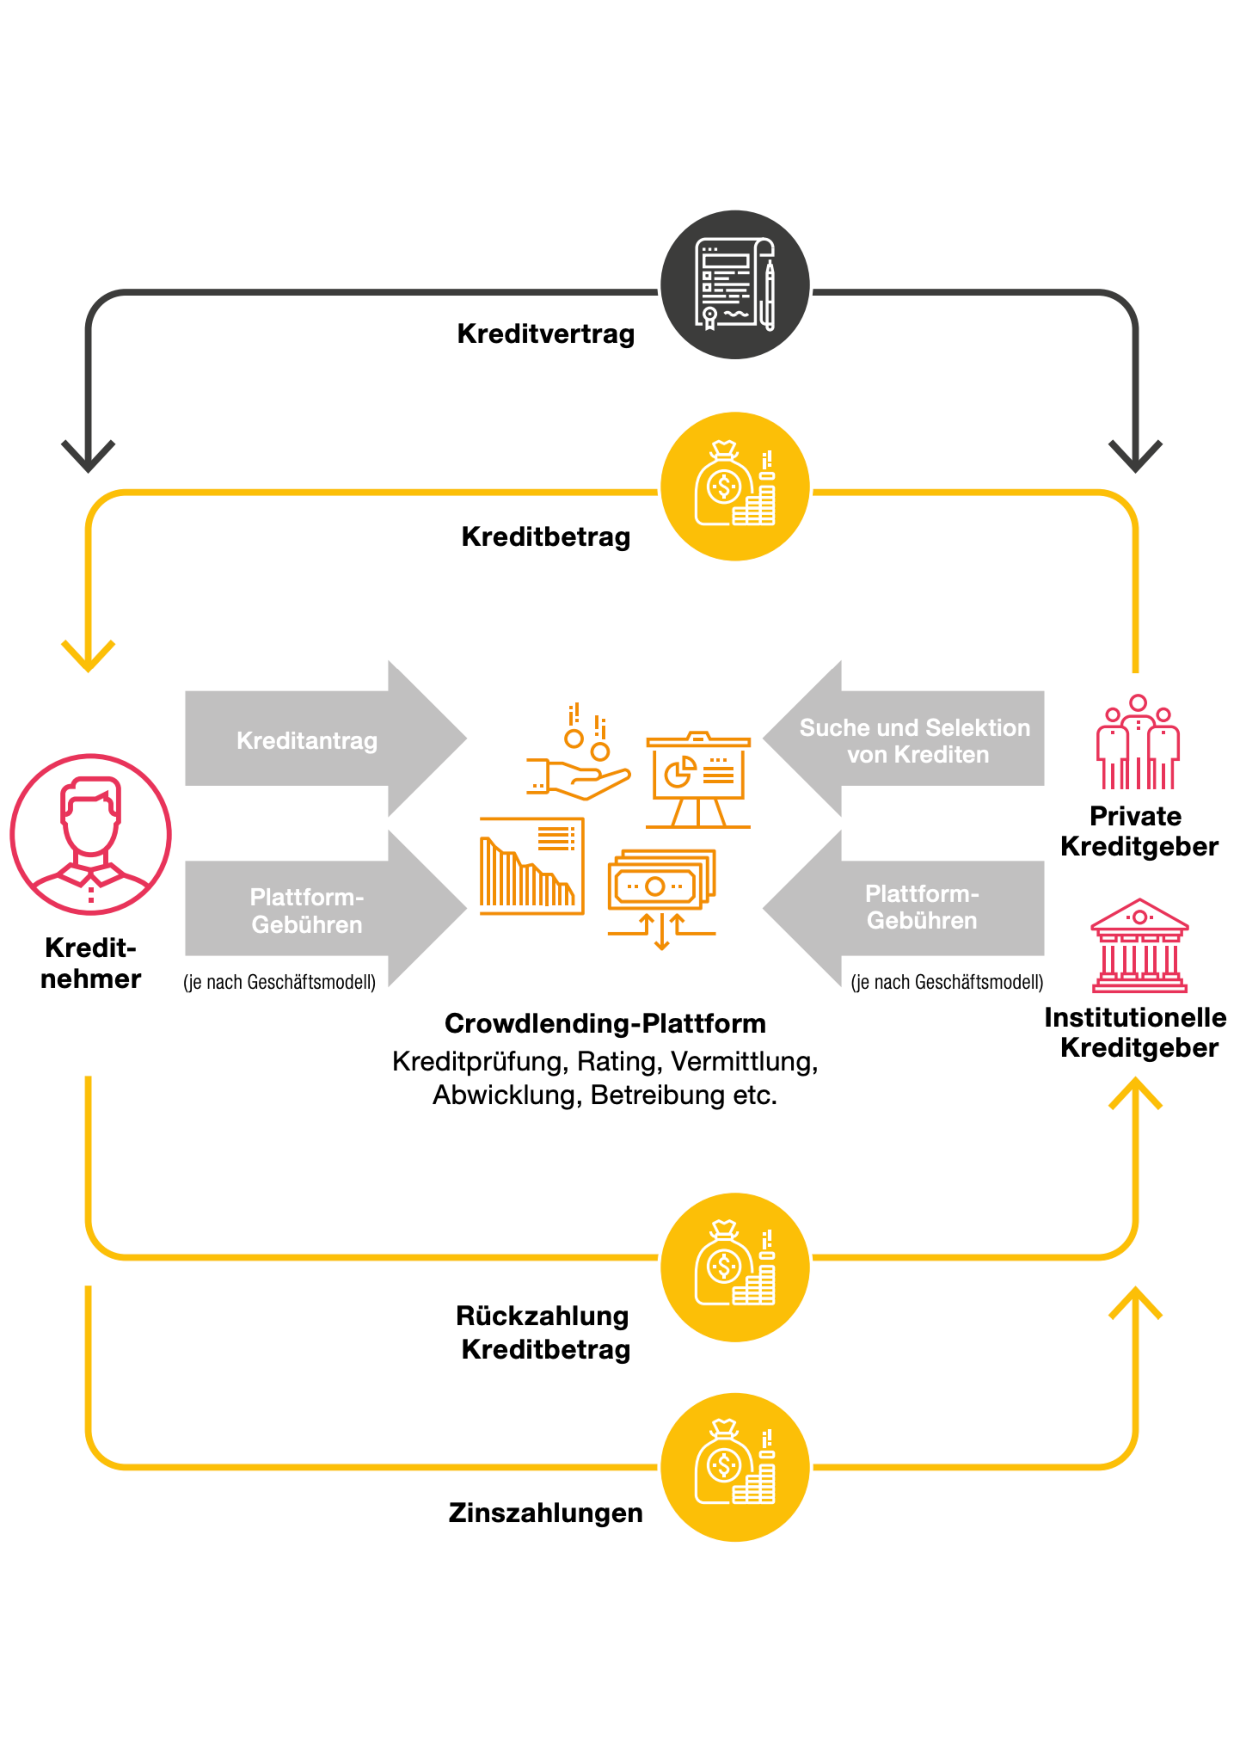
\includepdf[scale=.8,page=1,pagecommand=\section*{A. Funktionsweise Crowdlending\label{sec:A}}]{appendix/Crowdlending.pdf}
\end{appendix}

	
\end{document}
